\documentclass{article}

\usepackage{tikz}
\usepackage{lipsum}
\usepackage{graphicx}
\usepackage{subfigure}
\usepackage{enumitem}
\usepackage{tabu}
\usepackage{multirow}
\usepackage{amsmath}
\usepackage{amssymb}
\usepackage{epstopdf}
\usepackage{csquotes}
\usepackage{hyperref}
\usepackage{geometry}
\usepackage[sorting=none, backend=biber]{biblatex} 
\usepackage{subcaption}
\usepackage{caption}
\usepackage{fancyhdr}
\usepackage[UKenglish]{babel}
\geometry{a4paper, portrait, margin=3cm}
\usepackage{duckuments}
\usepackage[export]{adjustbox}
\usepackage{setspace}

\onehalfspacing 

\graphicspath{ {Images/} }

%graphicx normal mode settings
\def\gridspace{20}
\def\doublegridspace{40}
\def\griddiagonal{10}
\def\griddot{\circle*{2}}

\setlength{\parskip}{0.5em}


%\DeclareCaptionFormat{customCaptionFormat}
%{ 
%    \textbf{#1#2}\text{\small#3}
%}
%\DeclareCaptionFont{phv}
%{
%    \fontseries{n}\fontfamily{phv}\selectfont
%}
\captionsetup{font=sf,labelfont=bf}

%Header and Footer Stuff

% \author{Jason Thomas}
% \date{October 2025}

% \fancypagestyle{plain}{%  the preset of fancyhdr 
%     \fancyhf{} % clear all header and footer fields
%     \fancyhead[C]{\thedate}
%     \fancyhead[L]{\theauthor}
    %\fancyhead[R]{\the}
% }
\pagestyle{plain}

\addbibresource{articleReferences.bib}

% For indenting all lists
\newcommand{\newandsetlength}[2]{\newlength{#1}\setlength{#1}{#2}}

\newandsetlength{\doubleparindent}{4cm}
\setlist[description]{leftmargin=\doubleparindent,labelindent=\parindent}

% This is where your document will begin, after this anything you type should appear when compiled
\begin{document}

\begin{titlepage}
\begin{figure}[t!]
\centering

\includegraphics[width=5cm]{rmit-logo}
\end{figure}

\vspace*{2cm}

\begin{center}
{\large
	Probability of extinction for pathogens transmitted between ticks during co-feeding\\
	[1cm]
	A thesis submitted in fulfilment of the requirements for the degree of \\
    Bachelor of Science (Mathematics and Statistics) (Honours).\\
	[2cm]
	Jason Robert Thomas\\
	[0.5cm]
	Bachelor of Science (Mathematics and Statistics) \\
	[3cm]
	School of Science.\\
	[0.5cm]
	College of STEM.\\
	[0.5cm]
	RMIT University.\\
	[2cm]
	November 2025\\
}
\end{center}
	
\end{titlepage}


\section*{Declaration}
I certify that except where due acknowledgement has been made, the work is that of the author alone; the work has not been submitted previously, in whole or in part, to qualify for any other academic award; the content of the thesis is the result of work which has been carried out since the official commencement date of the approved research program; any editorial work, paid or unpaid, carried out by a third party is acknowledged; and, ethics procedures and guidelines have been followed. \\
[1cm]
Signed: Jason Thomas\\
[1cm]
Date: 29th of October, 2025\\

\section*{Acknowledgments}
I thank:
\begin{itemize}
\item Associate Professor Stephen Davis and Dr Simon Johnstone-Robertson for their supervision, feedback and advice during this project.
\item Dr Haydar Demirhan for his advice regarding statistical tests.
\item PhD candidate Daniel Longmuir, who helped me understand how to derive an important result.
\end{itemize}

\section*{Abstract}
Importance of tick-borne diseases (one or two sentences). \\
Aim of research (one sentence). \\
Methods (two sentences). \\
Results and findings (four or more sentences).

\newpage

\section*{Graphical abstract}

\begin{figure}[h!]
    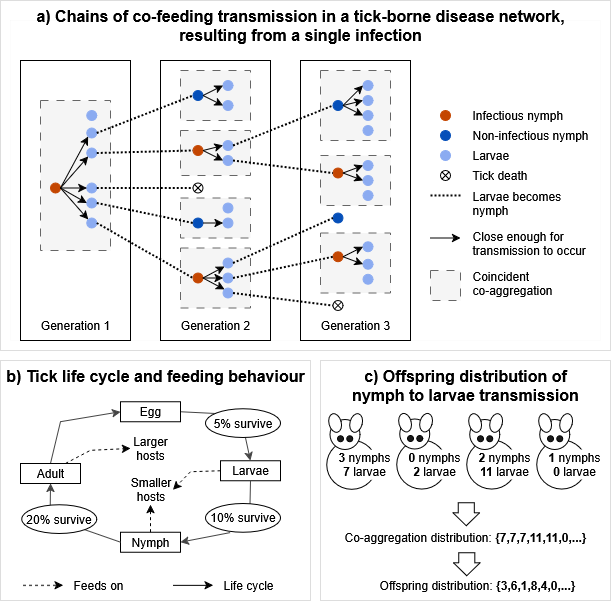
\includegraphics[width=0.99\textwidth, center]{Images/graphical_abstract_mk2.drawio}
    \caption{
    \textbf{a)} \textit{Branching process}. Co-feeding transmission  occurs when susceptible ticks (usually larvae) attach and feed in close proximity to one or more infectious ticks (usually a nymph) and acquire a pathogen directly. This project introduces simplifying assumptions about the situation in nature: i) all larvae are susceptible; ii) larvae and nymphs might co-aggregate on one host, but they might not be close enough for transmission to occur; iii) there are no other routes of transmission; iv) two larvae that become infectious nymphs will not co-feed on the same vertebrate. \\ 
    \textbf{b)} \textit{Life cycle}. This life cycle of ticks is: immature ticks are more plentiful, and that they tend to feed on small vertebrates \cite{Randolph1998}. This implies that immature ticks are largely responsible for co-feeding transmission. \\
    \textbf{c)} \textit{Offspring distribution}. An offspring distribution is needed when using a branching process simulation. We use this simulation to calculate the probability that a chain of transmissions, starting with just a single infectious tick, goes extinct. We introduce a method to derive the offspring distribution from commonly-collected tick burden data.
    }
\end{figure}

\newpage

\tableofcontents

\newpage

\section{Introduction}

Worldwide, tick-borne diseases (TBD) pose a significant health burden for humans and livestock. That is because ticks carry pathogens that can infect their vertebrate hosts when ticks take blood meals from their hosts. The pathogens that spread when ticks feed can cause diseases, and those diseases often have severe consequences for the individual vertebrate hosts that ticks feed on \cite{Johnson2023e}. This feeding behaviour allows for pathogens to spread either from tick-to-vertebrate-to-tick, or sometimes directly from tick-to-tick.

We can characterise and understand an individual tick's expected behaviour by its life stage. All tick species have four life stages: egg, larva, nymph and adult. During a tick's juvenile life stages - larvae and nymph - it will take blood meals from vertebrate hosts so that it can moult into its next life stage. Female adults will take a blood meal in order to produce eggs, but it will no longer moult \cite{Johnson2023a}.

When most ticks of a particular life stage feed on a small number of vertebrate hosts, then they are said to aggregate \cite{JohnstoneRobertson2020}. A necessary, but not sufficient, condition for co-feeding transmission to occur is the coincidence of larval and nymphal ticks aggregating on the same host \cite{Ferreri2014}, which is known as co-aggregation. When those ticks co-aggregate at the same time, then this is known as coincident co-aggregation. Field data frequently shows that coincident co-aggregation disproportionately affects only a fraction of the vertebrate host population, and the 80:20 rule is often cited for many parasites (including ticks), where 80\% of ticks can be found on just 20\% of vertebrate hosts \cite{Woolhouse1997}.

FIND A NEW PLACE FOR THIS PARAGRAPH... IF IT'S NEEDED
A TBD network is a web of transmissions: each edge is a transmission of a pathogen between individual ticks and their vertebrate hosts, and sometimes transmissions directly between individual ticks. TBD networks are complex; some networks of a single pathogen have multiple tick species and multiple host vertebrates \cite{Johnson2023e}. Ticks also exhibit different behaviours depending on seasonal variation \cite{Johnson2023k}. Adding to this complexity is multiple types of transmission, where systemic (tick-to-host) transmission is the most common and co-feeding transmission (tick-to-tick) is less-common \cite{HARRISON2012}.

\subsection{Tick biology}

Ticks are in the \textit{Arachnida} class of animals, as are spiders and mites. Ticks are diverse and widespread; the diversity of ticks, and the vertebrate hosts that they feed on, is greater where the climate is more tropical, however, ticks are found on all continents except Antarctica \cite{Johnson2023a}. There are three families of ticks described in research: \textit{Ixodidae} (Hard Ticks), \textit{Argasidae} (Soft Ticks) and \textit{Nuttalliellidae}. \textit{Ixodidae} has the most known genuses and about 700 species. \textit{Nuttalliellidae} has just one known species \cite{Nicholson2019}.

A tick species' family is indicative of its behaviour. \textit{Ixodidae} ticks take a single blood meal during each life stage, whereas \textit{Argasidae} ticks take multiple blood meals during each life stage \cite{Johnson2023d}. Nidicolous ticks are said to spend their lives in burrows, caves and nests that their hosts live in. Many species are said to be specialists and will target few species of vertebrate hosts. Some nidicolous species of ticks are host-specific. Many species of \textit{Ixodidae} ticks are said to be non-nidicolous and their typical habitats include forests, meadows and other clearings, grasslands, savannahs, and semi-desert or desert areas. Such species are often said to be generalists, meaning they take blood meals from a wide array of hosts \cite{Nicholson2019}. Most \textit{Argasidae} are nidicolous \cite{Vial2009}, while some \textit{Ixodidae} are nidicolous. 

This thesis will focus on species from the \textit{Ixodidae} family of ticks, which pose a more significant health concern for humans \cite{Parola2001}. Specifically, the analysis in this thesis will focus on \textit{Ixodes ricinus} and \textit{Ixodes trianguliceps}, for which we have data. \textit{I. ricinus} is said to be non-nidicolous while \textit{I. trianguliceps} is nidicolous \cite{Nicholson2019}.

The biology of \textit{Ixodidae} make them particularly competent vectors for many diseases. When they feed, they can stay attached for more than one week \cite{Johnson2023b}. Their extended period of feeding means that the transmission of pathogens is more likely to occur \cite{Gray2024}. They lack digestive enzymes, meaning that their midgut is relatively benign, which increases the probability of transstadial transmission. When they feed, they inject saliva into their hosts, which increases the chance of successful transmission \cite{Gray2024}.

Since nidicolous ticks such as \textit{I. trianguliceps} are specialists, then usually they are not directly a threat to humans or livestock. However, some nidicolous ticks will bite any vertebrate that comes into contact with their habitat. Otherwise, many nidicolous tick species could maintain a pathogen among a population of reservoir hosts \cite{gray2014}.

We can expect to find ticks of different lifestages in different frequencies and can expect them to feed on different vertebrate hosts. Given that ticks die during and between their life stages, then larvae are most abundant, nymphs less common, and adults less common still \cite{Randolph1998}. A tick's life stage will allow us to predict how it will feed. For \textit{I. ricinus}, adults tend to feed on larger vertebrate hosts, whereas immature \textit{I. ricinus} ticks will frequently feed on smaller vertebrate hosts \cite{Herrmann2015, Randolph1998}. In comparison, \textit{I. trianguliceps} will feed almost exclusively on small mammal hosts, and is regarded as a specialist \cite{Bown2003, Bown2008}.

Phenology:
- Tick activity by season
- Lifespan
- Preferred hosts
- Abundance of adult ticks M/F

\subsection{Tick-borne diseases}

Ticks harbour pathogens (viruses, bacteria and protozoa) that spread to vertebrate hosts when they take blood meals from those hosts. Those pathogens can cause diseases and many of those have severe health implications for vertebrate hosts, including humans \cite{Johnson2023e}.

\textit{I. ricinus} is the most important vector in central and western Europe, and is a vector for at least 20 pathogens, and at least eight pathogens that can affect humans, including Lyme disease and tick-borne encephalitis (TBE) \cite{Gray2024}. Pathogens transmitted by ticks are responsible for the majority of vector-borne disease in temperate North America, Europe and Asia, with Lyme Disease being the most prevalent tick-borne disease in the Northern Hemisphere \cite{Rochlin2020}. 

While the impact on human health is significant, so is the impact on the livestock industry. A recent paper estimated the cumulative impact on livestock due to TBD in India's dairy industry was \$787.63 million USD \cite{Singh2022}. A 2006 article reported that economic losses in Tanzania's cattle industry were estimated to be \$364 million USD \cite{Kivaria2006}.

The geographical ranges of \textit{I. ricinus} and \textit{I. trianguliceps} often overlap. \textit{I. ricinus} has been reported in all parts of Europe, including Iceland, and throughout Northern Africa \cite{Otranto_2017}. \textit{I. trianguliceps} has been reported across mainland Europe and in the British Isles \cite{Pf_ffle_2017}. This thesis includes data from a single forest where \textit{I. ricinus} and \textit{I. trianguliceps} were collected from small mammals trapped during a longitudinal field study \cite{Bown2008, Bown2011}.

The habitat of \textit{I. ricinus} is expanding in Europe, due to several factors. \textit{I. ricinus} has increased its altitudinal range, based on studies in Bosnia and Herzegovina, the Czech Republic and Slovakia \cite{Medlock2013}. Modelling suggests that under different climate change scenarios, the habitat of \textit{I. ricinus} will probably spread northwards in Northern Europe \cite{Alkishe_2017}. Other modelling shows a similar northward spread of \textit{I. ricinus}, although some southern regions of Europe are likely to become less suitable for \textit{I. ricinus}, and some other species of ticks \cite{Cunze_2022}. However, the spread of \textit{I. ricinus} is not due to climate change alone; other drivers include the expansion of tick host populations, anthropogenic factors and land use changes \cite{Medlock2013}.

There are three ways that a pathogen can spread through populations of ticks, as Harrison and Bennett explain in their 2012 article:
\begin{itemize}
	\item Female ticks may transmit the pathogen to eggs via transovarial transmission (vertical transmission).
	\item Nymphs may feed on, and infect, a host leading to a systemic infection; larval ticks may then acquire an infection by ingesting the blood of the infected host, \textbf{maintain the infection transstadially, and infect an alternative host during a subsequent blood meal as a nymph (systemic transmission).}
	\item Ticks may become infected by co-feeding, spatially or temporally, alongside infected ticks; this does not require the host to have a systemic infection but instead pathogens are passed from one tick to another as they feed together. This is referred to as co-feeding transmission \cite{HARRISON2012}.
\end{itemize}

In addition, for a tick-borne pathogen to survive in nature, it is necessary for ticks to transmit the pathogens onwards. However, that is not sufficient for the pathogen's survival. For a tick to become infected and then survive the moulting to then pass on the disease, the pathogen must survive transstadially; transstadial transmission is the maintenance of the pathogen between life stages \cite{Johnson2023d}. This is a feature of systemic, vertical and co-feeding transmission.

The importance of different transmission routes depends on the tick and host species. Co-feeding transmission is important in disease systems where vertebrate hosts are incompetent vectors for maintaining a pathogen \cite{HARRISON2012}. Several studies suggest that co-feeding transmission is required for TBE to persist in nature \cite{Hartemink2008, HARRISON2012}, but it is less important for the persistence of Lyme disease. Several studies on TBD show that co-feeding transmission will increase $ R_0 $, which is defined later in this introduction. \cite{JohnstoneRobertson2020, Rosa2003, Norman2004}. Some studies show that co-feeding transmission may allow a pathogen to persist even without systemic transmission \cite{Rosa2003, Norman2004}. The focus of this thesis is on such a scenario.

If an \textit{Ixodidae} larva becomes infected during a blood meal (either via systemic or co-feeding transmission), then it transmitting the pathogen is not guaranteed. It must first survive the moulting process to become a nymph. It must then find another vertebrate host to feed upon. If the pathogen survives transstadially, then further transmission is possible. For the species \textit{I. ricinus}, commonly called a deer tick or sheep tick, the larva-to-nymph moulting success rate was reported at 91.9\% under some laboratory conditions \cite{Hurry2021}. Research from 2016 suggested that larvae-to-nymph moulting success of \textit{I. ricinus} was dependent on environmental conditions, with evidence to suggest that snow cover would act as a temperature buffer during Germany's winter \cite{Dautel2016}. For the species \textit{I. trianguliceps}, mortality from larvae to nymph is density-dependent \cite{Randolph1994}.

\subsection{The definition and importance of \texorpdfstring{$ R_0 $}{R0}}

The most important and widely-used concept in modelling transmissible diseases is the basic reproduction number $ R_0 $. This is a frequently-cited concept across epidemiology, and can be defined as the mean number of new infections per infection in an entirely susceptible population \cite{Diekman2000}. \textbf{It differs from the effective reproductive number $ R_t $}, which is used to quantify the efficacy of control measures in real time \cite{Lim2020}. Taken together, research sometimes uses the term $ R $ to indicate the reproductive number at different stages of an outbreak \cite{Jewell2022}.

A disadvantage of using $ R_0 $, which is a notion of generational growth, is that it does not describe growth in real time. During the early stages of an outbreak in a susceptible population, we can understand growth as being exponential:

\begin{equation}
	I(t) \approx Ce^{rt}
\end{equation}

where $ I $ is the total number of infections up until time $ t $, $ C $ is some constant, and $ r $ is the real time growth rate \cite{Diekman2000}.

$ R_0 $ is not a rate and is dimensionless, however, it has a relationship with the real-time growth rate, $ r $ \cite{Diekman2000}:

\begin{align}\label{R0}
  R_0 < 1 &\iff r < 0 \nonumber \\
  R_0 > 1 &\iff r > 0
\end{align}

In other words, the outbreak will undergo exponential decay when $ R_0 < 1 $, but an outbreak can be expected to persist when $ R_0 > 1 $. An important nuance is that $ R_0 > 1 $ is a necessary but insufficient condition for an outbreak to persist; due to stochasticity, the disease may still become extinct, even if $ R_0 > 1 $. This thesis will concentrate on $ R_0 $, rather than $ R_t $, because we assume that populations of ticks are entirely susceptible when a single infected tick is introduced.

Determining $ R_0 $ for wildlife disease systems often involve added complexities. Individual host species and individuals themselves have different susceptibilities, infectivity, and contacts. Given that an individual tick has different life stages, then these differences can exist within an individual throughout its life. Adding to the complexity is multiple transmission routes for many disease systems \cite{Hartemink2008}.

Structured population models allow for modelling these complexities; next-generation matrices can help model systemic transmission and systems with multiple species and transmission routes \cite{Diekman2000}. However, this thesis investigates the particular case where only co-feeding transmission is possible. Therefore, $ R_0 $ in this thesis is simply the average number of new infections per infection. Finding $ R_0 $ in previous research has involved using contact trace data \cite{LloydSmith2005}, and this thesis introduces a method to simulate that data based on tick aggregation data.

\subsection{Heterogeneity in disease networks}

The extent to which individuals infected with transmissible diseases are able to infect their peers varies with by multiple factors, including the specific disease, host population and environmental factors \cite{LloydSmith2005}. In transmissible disease systems, heterogeneity in individual behaviour can mean that some of the infected will not transmit the disease at all, while some might infect many of their peers. 

To understand the differences in individual behaviour, the 80:20 rule is often cited. This is where 80\% of cases are caused by 20\% of infected individuals. Many vector-borne and sexually-transmitted diseases follow the 80:20 rule. \cite{Woolhouse1997}. When larvae and nymphs aggregate on the same vertebrate hosts, they are said to co-aggregate. There is significant evidence to suggest that heterogeneity exists in TBD systems, and that co-aggregation data follows the 80:20 rule \cite{Ferreri2014, Brunner2008, HARRISON2012, JohnstoneRobertson2020}. In the sense that many ticks feed on just a fraction of the available vertebrates. 

While it is true that some infected individuals will come into contact with more of their peers, and are in a sense "super-spreaders", it is also true that some individuals have a higher infectiousness and are "super-sheaders" \cite{VanderWaal_2016}.

- individual reproductive number
q
- using the NB distribution

 then SOMETHING ABOUT SUPERSPREADING.



It is widely-recognised that individual behaviour varies. Important research in 2005 made the case that superspreading events are normal events in the spread of infectious diseases \cite{LloydSmith2005}. 



BELOW, SHOULD THIS BE MOVED TO THE SECTION ON THE BRANCHING PROCESS SIMULATION? Classically, models of disease outbreaks have assumed homogeneity in individual infectiousness and behaviour \cite{Garske2008}. These have typically been compartment models; the Susceptible-Infectious-Recovered systems of ordinary differential equations are common, although they can take many forms with more compartments defined. An assumption of those models is that the compartments are each large enough that the behaviour of individuals in those compartments is homogeneous. This is an appropriate assumption once an outbreak is established. However, at the start of an outbreak, the number of infectious individuals must be small. This exposes a limitation: compartment models that lack a stochastic element are insufficient to describe the very early stages of an outbreak \cite{Brauer2008a}. One approach is to use the SIR modelling framework to define stochastic differential equations \cite{Allen2017}, but there are other stochastic methods available. But, in any population, the degree infectiousness is distributed continuously, which further impedes our ability to divide a population into homogenous subgroups. This thesis addresses the heterogeneity that occurs in TBD systems by using a branching process simulation, which is defined in a later section.

The Perato rule, or 80/20 rule, is a useful concept to a variety of disease systems. .... ALL THE STUFF ABOUT 80/20 ... However, for directly-transmitted disease systems, the infectiousness of each case is a complex mix of host, pathogen and environmental factors \cite{LloydSmith2005}. That led Lloyd-Smith and others to define an individual reproductive number, which is introduced and defined later.






However, co-aggregation is not sufficient to guarantee transmission, and an outbreak may still go extinct. This thesis addresses that uncertainty by introducing a stochastic process to 

The negative binomial distribution is a very useful tool in the study of heterogeneity in count data: 


The work of Lloyd-Smith and others in 2005 showed that the Negative Binomial (NB) distribution was a better fit than either the Poisson or Geometric distributions to many contact trace and surveillance datasets; this is an important result that this thesis will reproduce. Prior to 2005, there was already evidence of superspreading in disease networks. Data from the early-2000s SARS epidemic in Singapore showed that five individuals were identified as superspreaders \cite{CDC2003} after infecting another 103 individuals.

Many vector-borne and sexually-transmitted diseases follow the 80/20 rule: 80\% of cases are caused by 20\% of infected individuals \cite{Woolhouse1997}.


The NB distribution has become the de-facto choice for tick aggregation data, and for parasite aggregation data more generally. In 1998, Shaw et al showed that the NB distribution was an appropriate fit for 90\% of datasets that they looked at \cite{SHAW1998}. Many articles concerning tick aggregation data have used NB distribution \cite{Bown2003, HARRISON2012, Brunner2008}. Other work suggests that when tick aggregation data has a heavy right tail, which indicates extreme heterogeneity in vectors on hosts, then the Power-Law distribution is a better fit \cite{Ferreri2014, Bisanzio2010} for some purposes.

\subsection{Thinking about TBD transmission using contact networks}

Network thinking can help overcome some of the problems associated with deterministic models; network models allow for representing the heterogeneity that exists in individual behaviour. Simulations suggest that stochastic methods lead to lower estimates for $ R_0 $ \cite{Brauer2008b}.

When taking a network approach, a common technique  is to define a contact network. This is a graph where vertices represent individuals and edges between them represent contacts. Those contacts may also facilitate transmission. The number of edges that connects one vertex to its neighbours is called the vertex's degree. The degree distribution for the graph is  $ \{ p_k \} $  \cite{Brauer2008b}. For a vector-borne disease, a bipartite graph is useful to represent contacts between vectors and hosts.

In 2010, Bisanzio et al modelled the potential spread of TBE and Lyme disease. Their analysis was for co-aggregation data for \textit{I. ricinus}. They made a bipartite contact network to represent the potential for transmission between vectors and hosts. Their analysis showed that extreme aggregation on hosts would greatly impact the epidemic threshold \cite{Bisanzio2010}. Their analysis used bipartite networks with edges between hosts and vectors, but edges between vectors to represent transovarial transmission had no effect on the outcome. They used an SIS (susceptible-infected-susceptible) model to measure the epidemic threshold's dependence on the network size.

In 2016, the work of Ferreri et al followed the work of Bisanzio et al, in that they also applied an SIS model to the contact network data. Their model represented aggregation as star graphs, with vertebrates at the centre and ticks as peripheral nodes. These are constellation graphs. The model randomly re-attaches tick nodes to new constellations. Their analysis focused on co-feeding transmission, but the model did not differentiate between the different life stages of tick.

In 2020, the work of Johnstone-Robertsone et al characterised a tick-host contact network as a directed, acyclic, bipartite graph. The ticks represent one node, but the edges leading away from the vertebrate host node $ k_{out} $ represent the number of larvae that co-aggregate, and $ k_{in} $ represent the number of nymphs that co-aggregate. However, there is only one node per tick. This implies that the tick nodes represent a tick in its larval and then nymphal life stages. Johnstone-Robertson et al then superimposed a transmission network; co-feeding (edges between ticks) and systemic (edges from tick-to-host, host-to-tick) \cite{JohnstoneRobertson2020}. This work is the main inspiration for the method, which is presented later in this thesis, of simulating outbreaks by using co-aggregation data.

\subsection{Galton-Watson Branching Processes}

A Galton-Watson Branching Process (GWBP) is a useful device for analysing how a disease spreads \cite{Diekman2000}, but its original use was concerned with the extinction of families in Victorian Britain \cite{Athreya1972}. Whether a family becomes extinct because each father has no sons to carry on the family name, or a disease outbreak becomes extinct because each infected person infects no one else, are very similar problems.

GWBP are single-type branching processes and are discrete-time Markov chains; the number of offspring in generation $ n $ depends on the number of individuals in generation $ n - 1 $, but not on previous generations \cite{Allen2019}.

An offspring distribution is a discrete random variable that represents the number of new infections per infection; a candidate offspring distribution must be selected to use a branching process.

Let $ p_k $ be a discrete random variable for how many new infections there will be, and $ \sum_{k=0}^\infty p_k =  1  $ \cite{Diekman2000}.

The probability generating function is:

\begin{equation}\label{BranchingProcess}
    g(z) = \sum_{k=0}^\infty p_k z^k, |z| \le 1
\end{equation}

Now, let $ z_n $ be the probability that the chain is extinction after $ n $ generations. Then substitute $ z_n = g(z_{n-1})$

\begin{equation}\label{BranchingProcess2}
    z_{n} = g(z_{n-1}) = \sum_{k=0}^\infty q_k (z_{n-1})^k
\end{equation}

This indicates that $ g $ increases as $ z_n $ increases. But since all $ |z_n| \le 1 $, then this series converges. That leads to the simplification $ z = g(z) $. Later, we use this result to approximate the probability of extinction to within some tolerance of error.

Diekman and Heesterbeek, in their 2000 text, describe this as taking into account demographic stochasticity \cite{Diekman2000}.

\subsection{Multi-type branching processes for modelling TBD}

The single-type branching process defined previously is useful when offspring are the same type as their parent \cite{Allen2019}. However, many disease systems can be modelled using a multitype branching process. These simulations are capable of representing more complex transmissions than just one pathogen and one species of host.

In 2017 Maliyoni and others showed that a multitype branching process simulation was useful modelling systemic transmission between \textit{Amblyomma americanum} ticks and \textit{Odocoileus virginianus} deer. Their technique used a deterministic ODE approach to calculate the $ R_0 $. They then calculated the probability of extinction using a multitype branching process. Their study targeted the pathogen \textit{Ehrlichia chaffeensis}, which is the causative agent of \textit{human monocytic ehrlichiosis}. The study compared the predictions made using the deterministic and stochastic models and found deterministic models would predict a stable equilibrium if $ R_0 > 1 $, whereas the stochastic models would sometimes still lead to disease extinction even if $ R_0 > 1 $.

The same authors, in 2019, published an article that modelled the spread of multiple pathogens via co-feeding and trans-ovarial transmission. The study looked at pathogens \textit{Rickettsia parkeri} and \textit{Rickettsia amblyommii}, for which \textit{A. americanum} is a vector. That study also used a multitype GWBP to estimate the probability of pathogen extinction.

\subsection{Use of the individual reproductive number}

As previously-mentioned, the work by Lloyd-Smith et al was influential. Their article was notable because it proposed a protocol to define a superspreading event, and showed that superspreading was a normal feature of disease spread \cite{LloydSmith2005}.

Their article is relevant for TBD because it introduced the concept of an individual reproductive number. The use of GWBP analyses for investigating infectious disease was established before the 2005 article was published. However, the paper included heterogeneity in individuals' ability to transmit the virus by using a Poisson process. When the parameter of the Poisson distribution, $ v $, is itself a random variable then the resulting Poisson mixture is a Negative Binomial distribution:

\begin{align}\label{PoissonMixture}
    v &\sim \text{Gamma}\left(R_0, \frac{R_0}{k}\right) \nonumber \\
    Z &\sim \text{Poisson}(v) \\
    Z &\sim \text{NegBinom}(R_0, k) \nonumber
\end{align}

The article also fit multiple discrete distributions (Poisson, Geometric and Negative Binomial) and found that the Negative Binomial distribution was usually the better fit, although the Poisson and Geometric distributions are special cases of the Negative Binomial distributions. This indicates that individual heterogeneity is present in real-world disease systems.

An important nuance is that the individual reproductive number was introduced and applied to disease systems that spread between humans, and that humans have individual reproductive histories that affect their current reproductive capacity. Lloyd-Smith and others detailed how environmental factors - like people being on planes or in hospitals - could affect their individual ability to transmit a pathogen.

This thesis uses the assumption that individual ticks have varied individual reproductive capacities, as do humans in human disease networks.  

\newpage

\section{Research project}

\subsection{Aims}

\begin{itemize}
  \item Implement a technique, which we believe is novel, to generate an offspring distribution by using tick burden data, which field ecologists commonly-collect. An offspring distribution is required to use a GWBP simulation.
  \item Publish and document the use of a new method for use by TBD researchers, who may wish to calculate the probability that a TBD goes extinct, where co-feeding is the only viable transmission route.
  \item Find estimates for parameters to be used as a threshold; passing the threshold would be necessary, but not sufficient, for a tick-borne pathogen to persist in nature via co-feeding transmission alone. Parameters below the threshold would necessarily cause extinction.
\end{itemize}

\subsection{Methods}

\begin{enumerate}
  \item Analyse and summarise provided tick co-aggregation datasets. 
  \item Reproduce results from an important paper that simulates extinctions of directly-transmitted disease chains. Then, apply these extinction simulations to simulated TBD networks, where co-feeding transmission is a form of direct transmission.
  \item Implement a parameterisation of the Negative Binomial distribution that uses that simulated offspring distribution’s sample mean as a shape parameter. This is currently not supported in Python’s SciPy. This will be one candidate Offspring Distribution.
  \item Use the co-aggregation data to derive offspring distributions, which is required for the GWBP analysis, for each species of tick to determine the probability that a chain of transmissions becomes extinct.
  \item Fit the reparameterised Negative Binomial, Geometric and Poisson distributions to each subset of data, as candidates for offspring distributions. Use a goodness of fit method to check which distribution best-fits each subset of data.
  \item Once we have a candidate offspring distribution for each tick species, use the theory of branching processes to find the probability of pathogen extinction based on given starting parameters.
  \item Ensure all code is documented, easy to read and usable for future researchers. Ensure code is published online for others to use.
\end{enumerate}

\subsection{Expected outcomes}

\begin{itemize}
  \item The Negative Binomial distribution will be a better fit for simulated offspring data, when compared with Poisson and Geometric distributions.
  \item Some combinations of parameters will allow for $ R_0 > 1 $, indicating that co-feeding transmission might be sufficient to maintain some combinations of: pathogen, tick, and vertebrate host species, in different environmental conditions.
  \item A single-type GWBP may be too simple, and there will be a cause to recommend a multi-type GWBP simulation in future research. We can expect this to feature in the discussion section of this thesis.
\end{itemize}

\newpage

\section{Summaries of Kielder Forest data}

This project makes use of data provided by **INSERT** Kevin Bown. The **INSERT** collected that data in the Kielder Forest in the United Kingdom between April and August in 2004 and 2005. The provided dataset presents the numbers of larvae and nymphs found on each vertebrate. Vertebrates were included in the collection once only.

The analysis by Bown et al originally **INSERT DETAILS ABOUT WHY THEY COLLECTED THE DATA, HOW, ETC**.

The data includes only the tick species \textit{I. trianguliceps} and  \textit{I. ricinus}. The host species were mostly "field voles", (\textit{Microtus agrestis}), and "common shrews" (\textit{Sorex araneus}). The researchers also encountered small numbers of other small mammals. The common shrew and field voles vastly outnumber other vertebrate hosts in the Kielder Forest data. The use of that data in this project focuses on the common shrew and field vole observations. 

Of interest is whether larvae and nymphs of a particular tick species have the same seasonal variation in activity. If the larvae and nymphs are active at different times, then the opportunity for co-feeding transmission to occur is limited. Seasonal activity for nymphs and larvae, for \textit{I. ricinus} and \textit{I. trianguliceps}, collected at the Kielder Forest is presented in Figure \ref{fig:kielder_seasonal}.

\begin{figure}
	\centering
	\begin{tabular}{ll}
		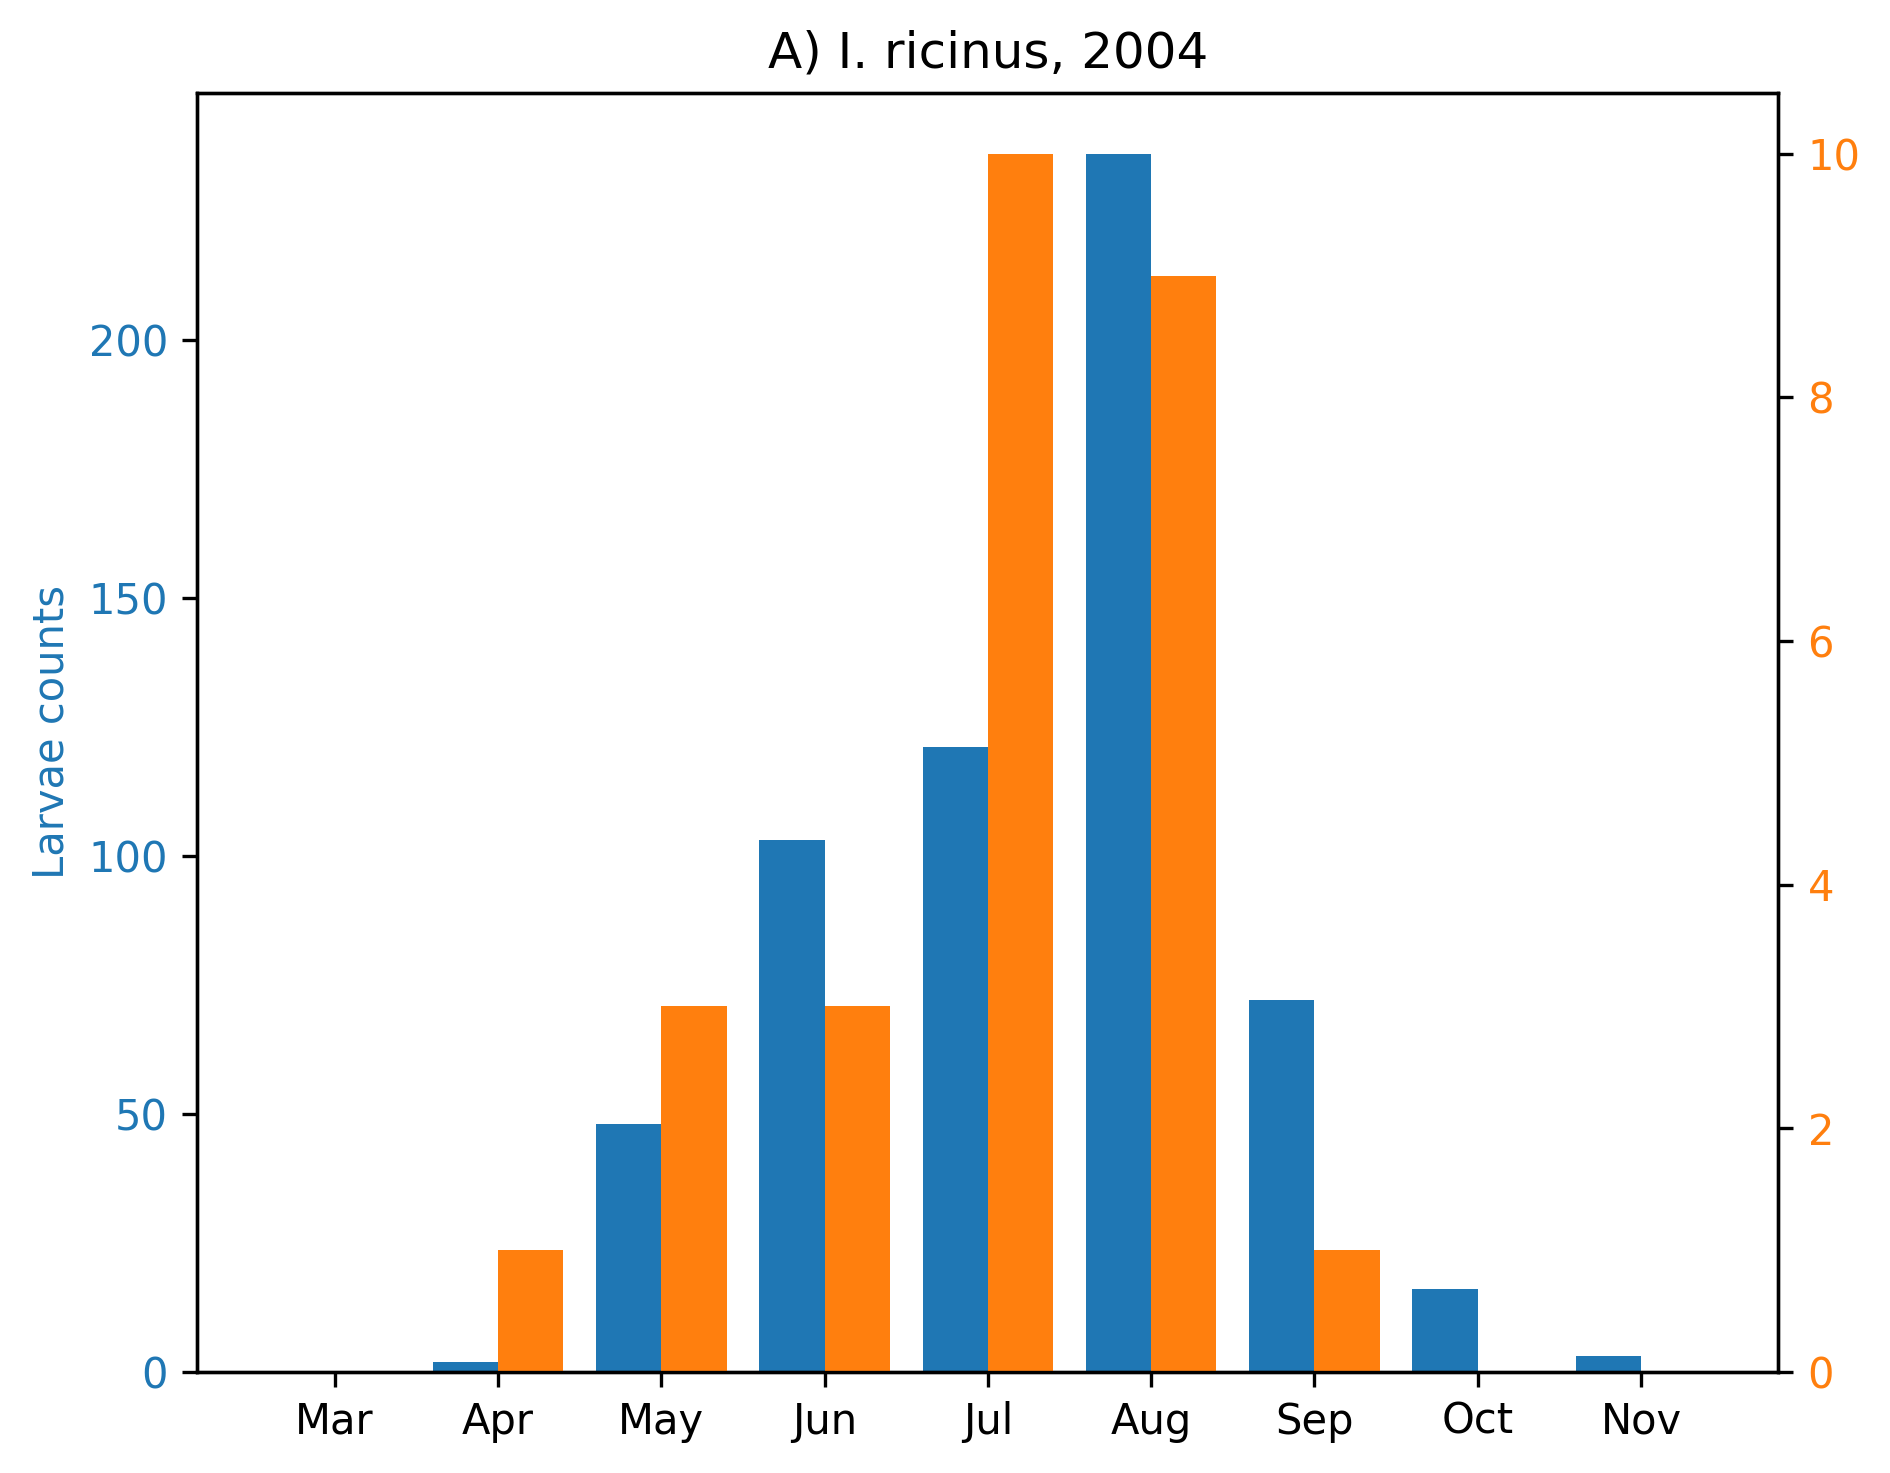
\includegraphics[width=.5\linewidth,valign=m]{A) I. ricinus, 2004} & 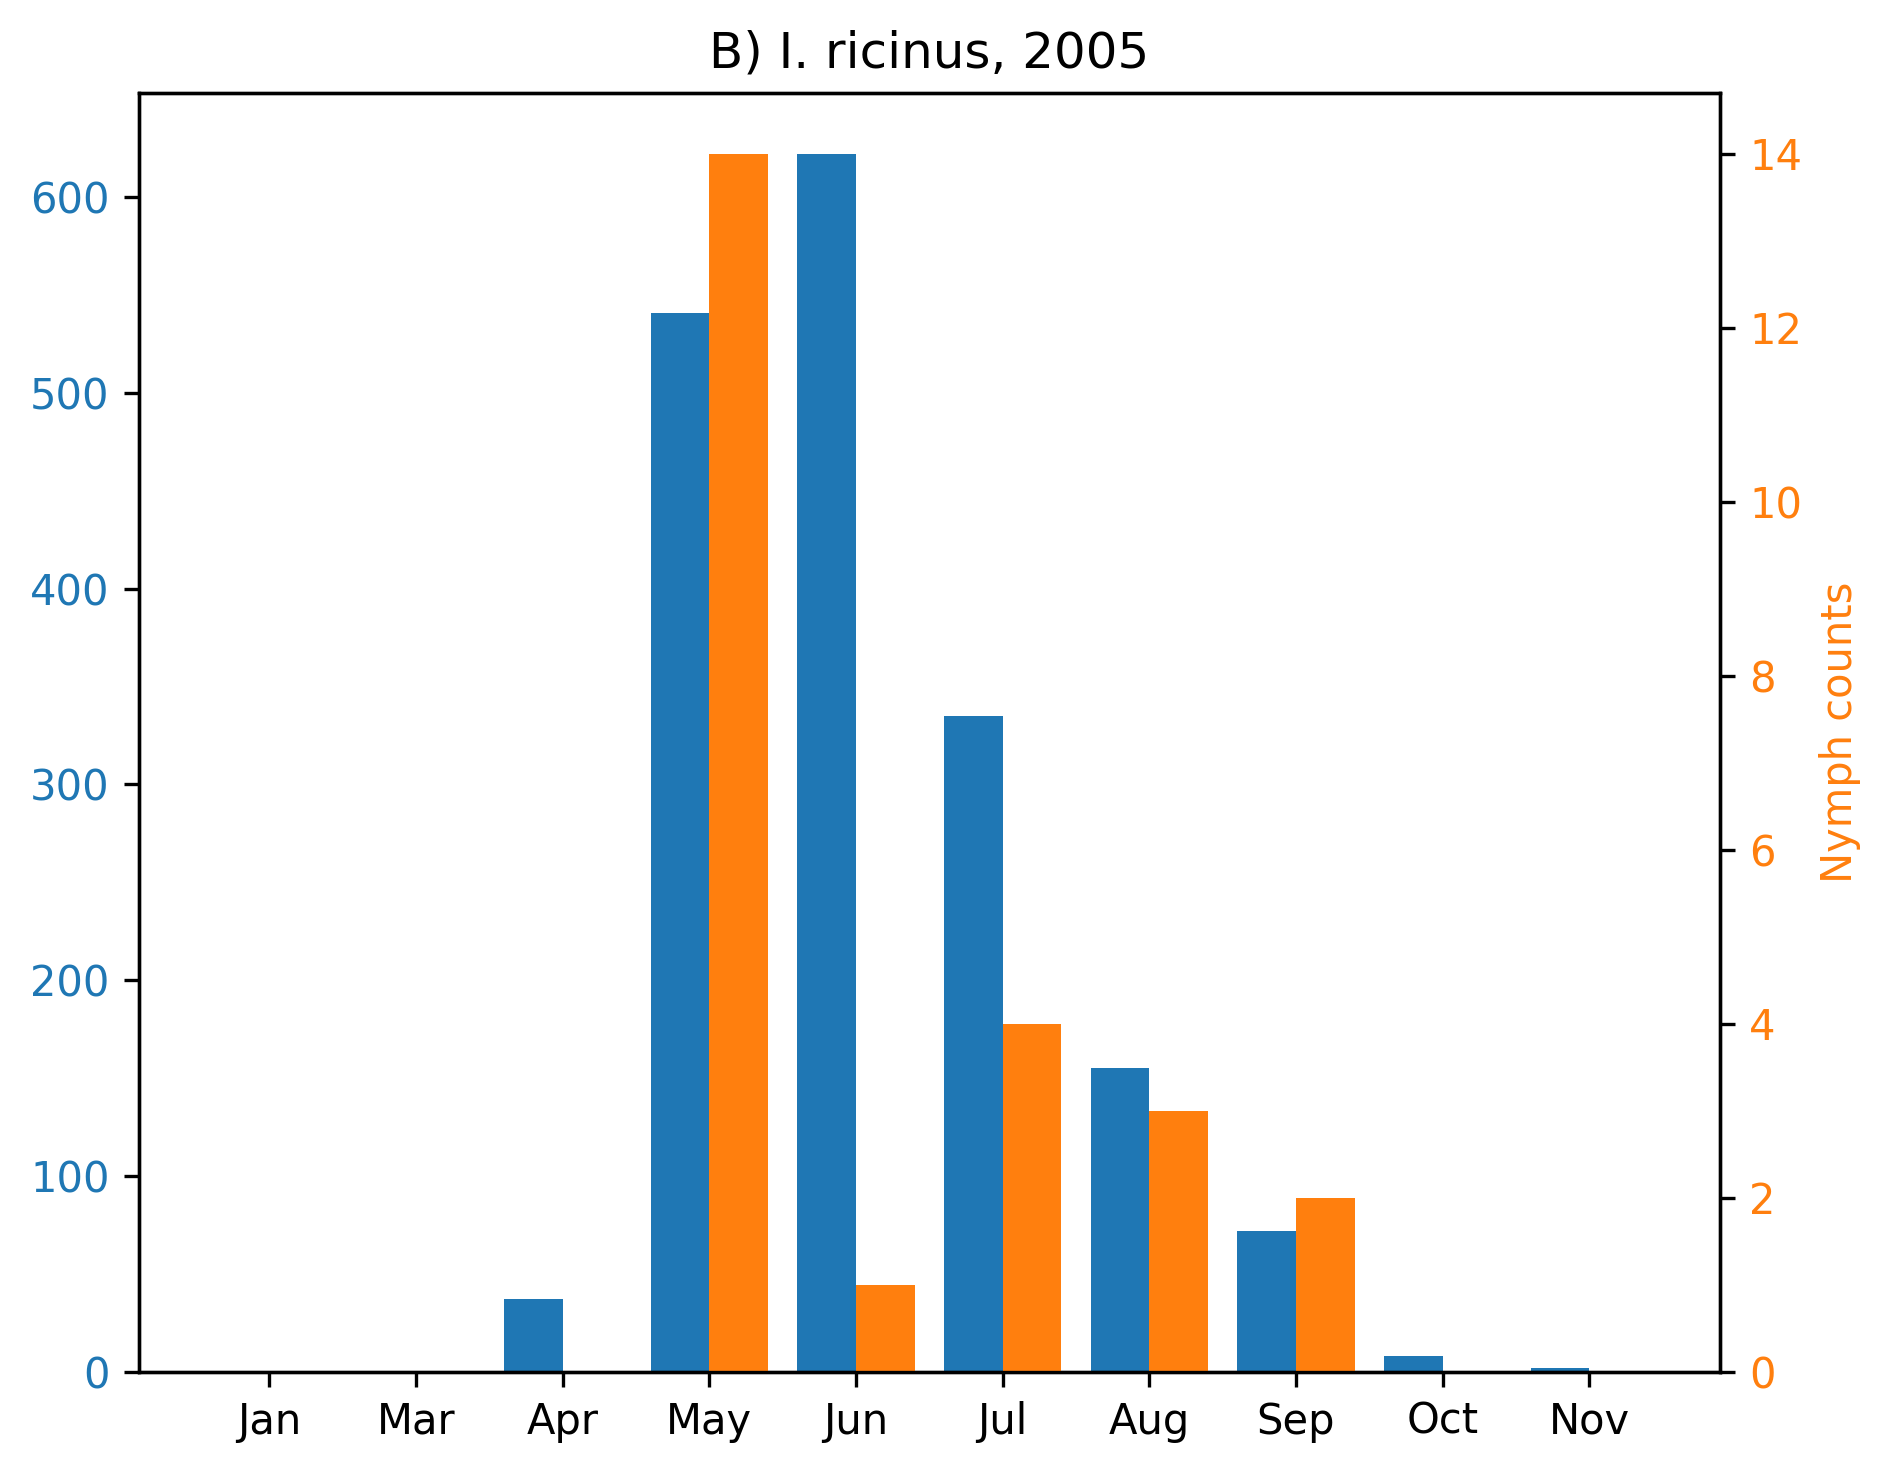
\includegraphics[width=.5\linewidth,valign=m]{B) I. ricinus, 2005} \\
		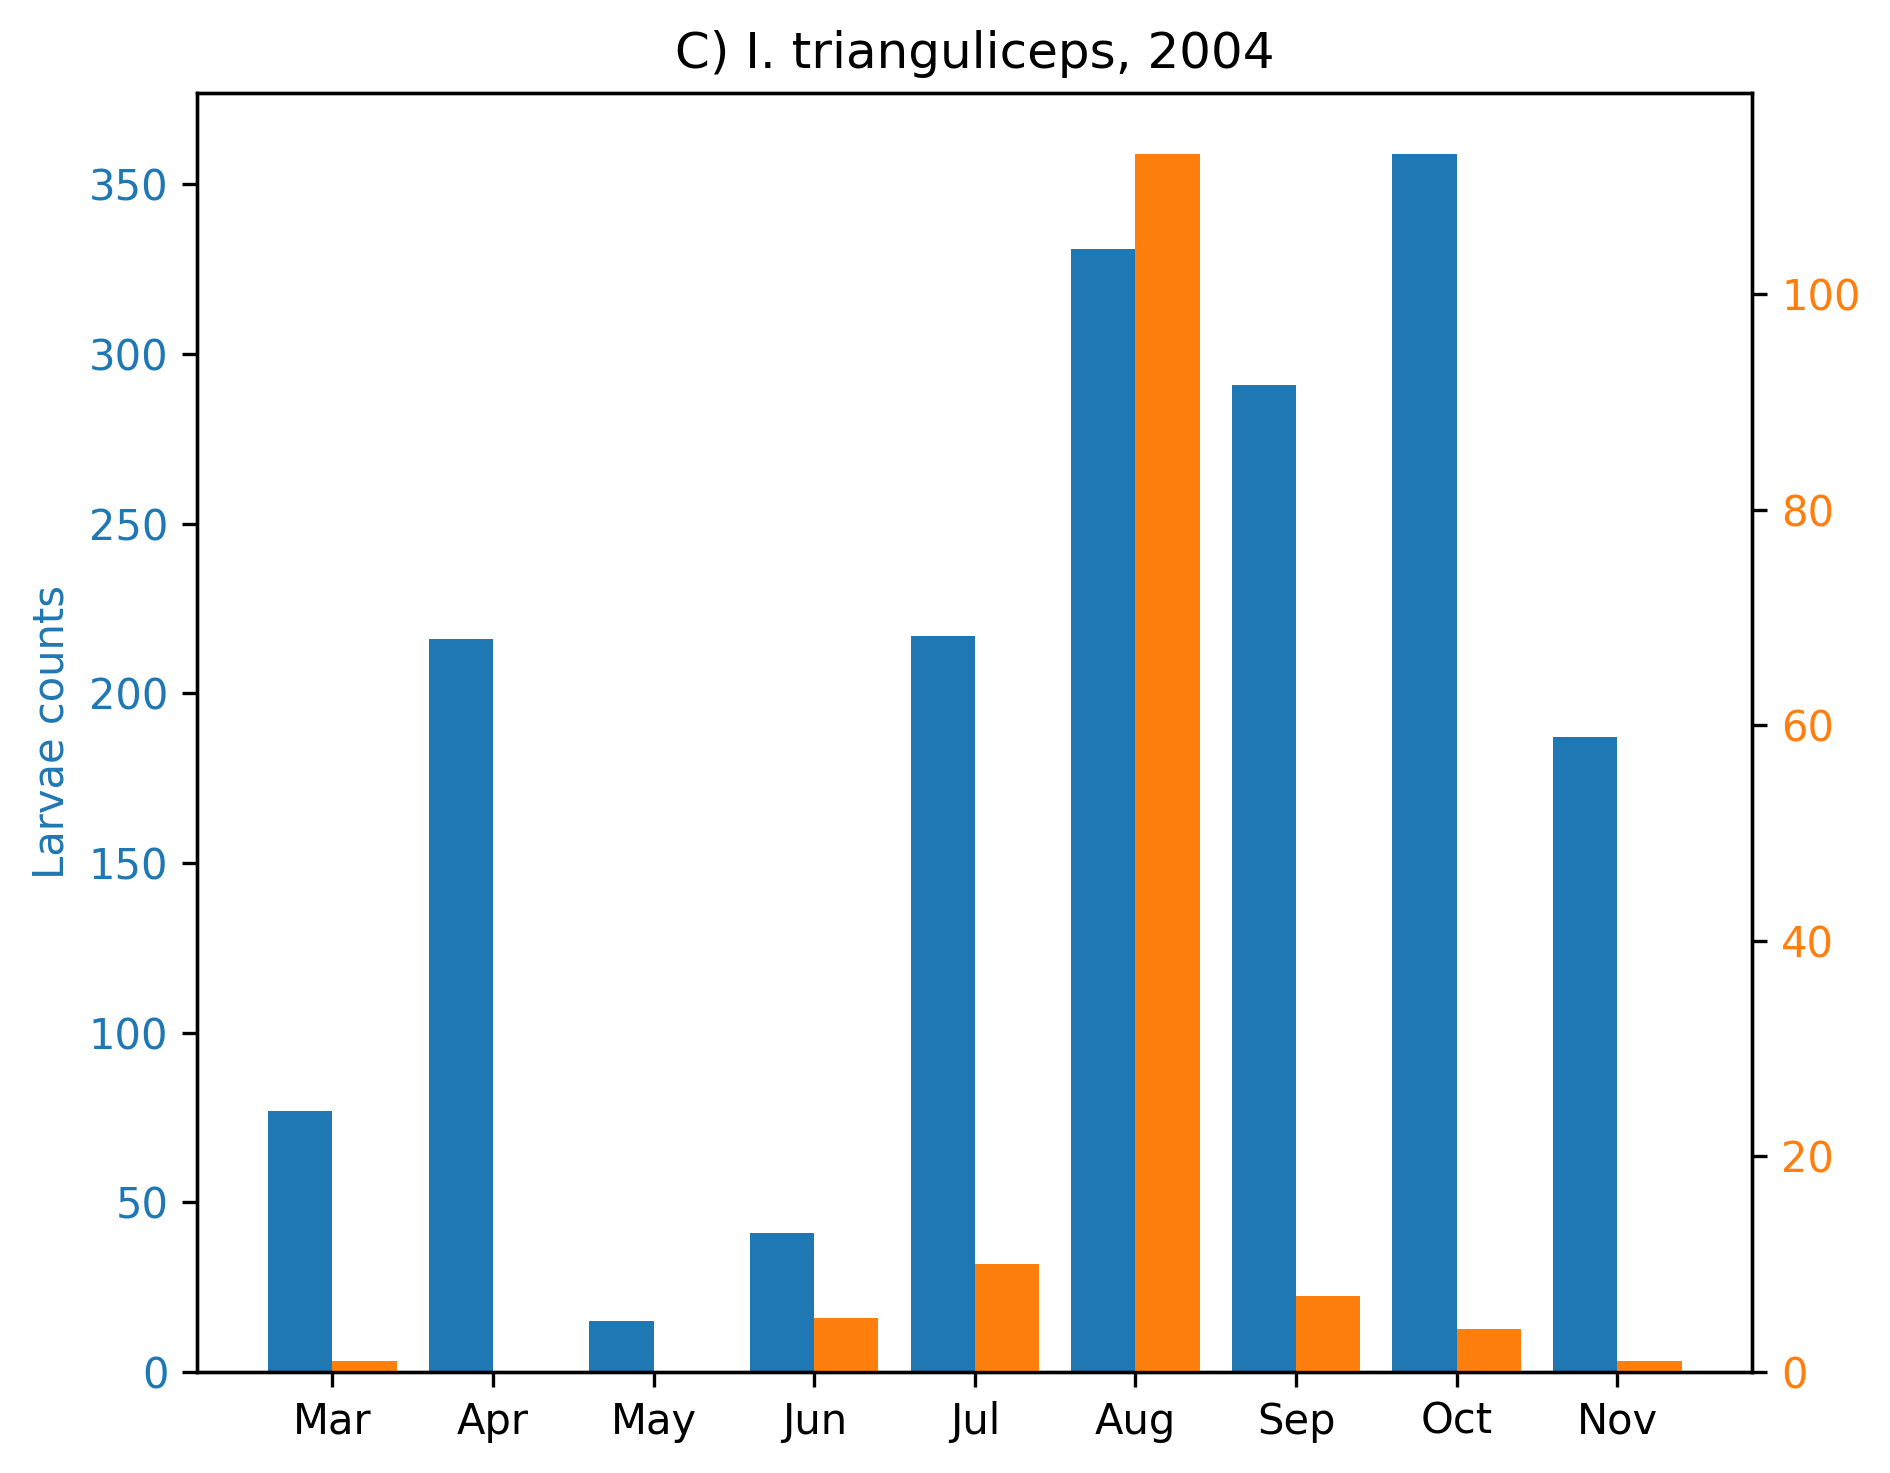
\includegraphics[width=.5\linewidth,valign=m]{C) I. trianguliceps, 2004} & 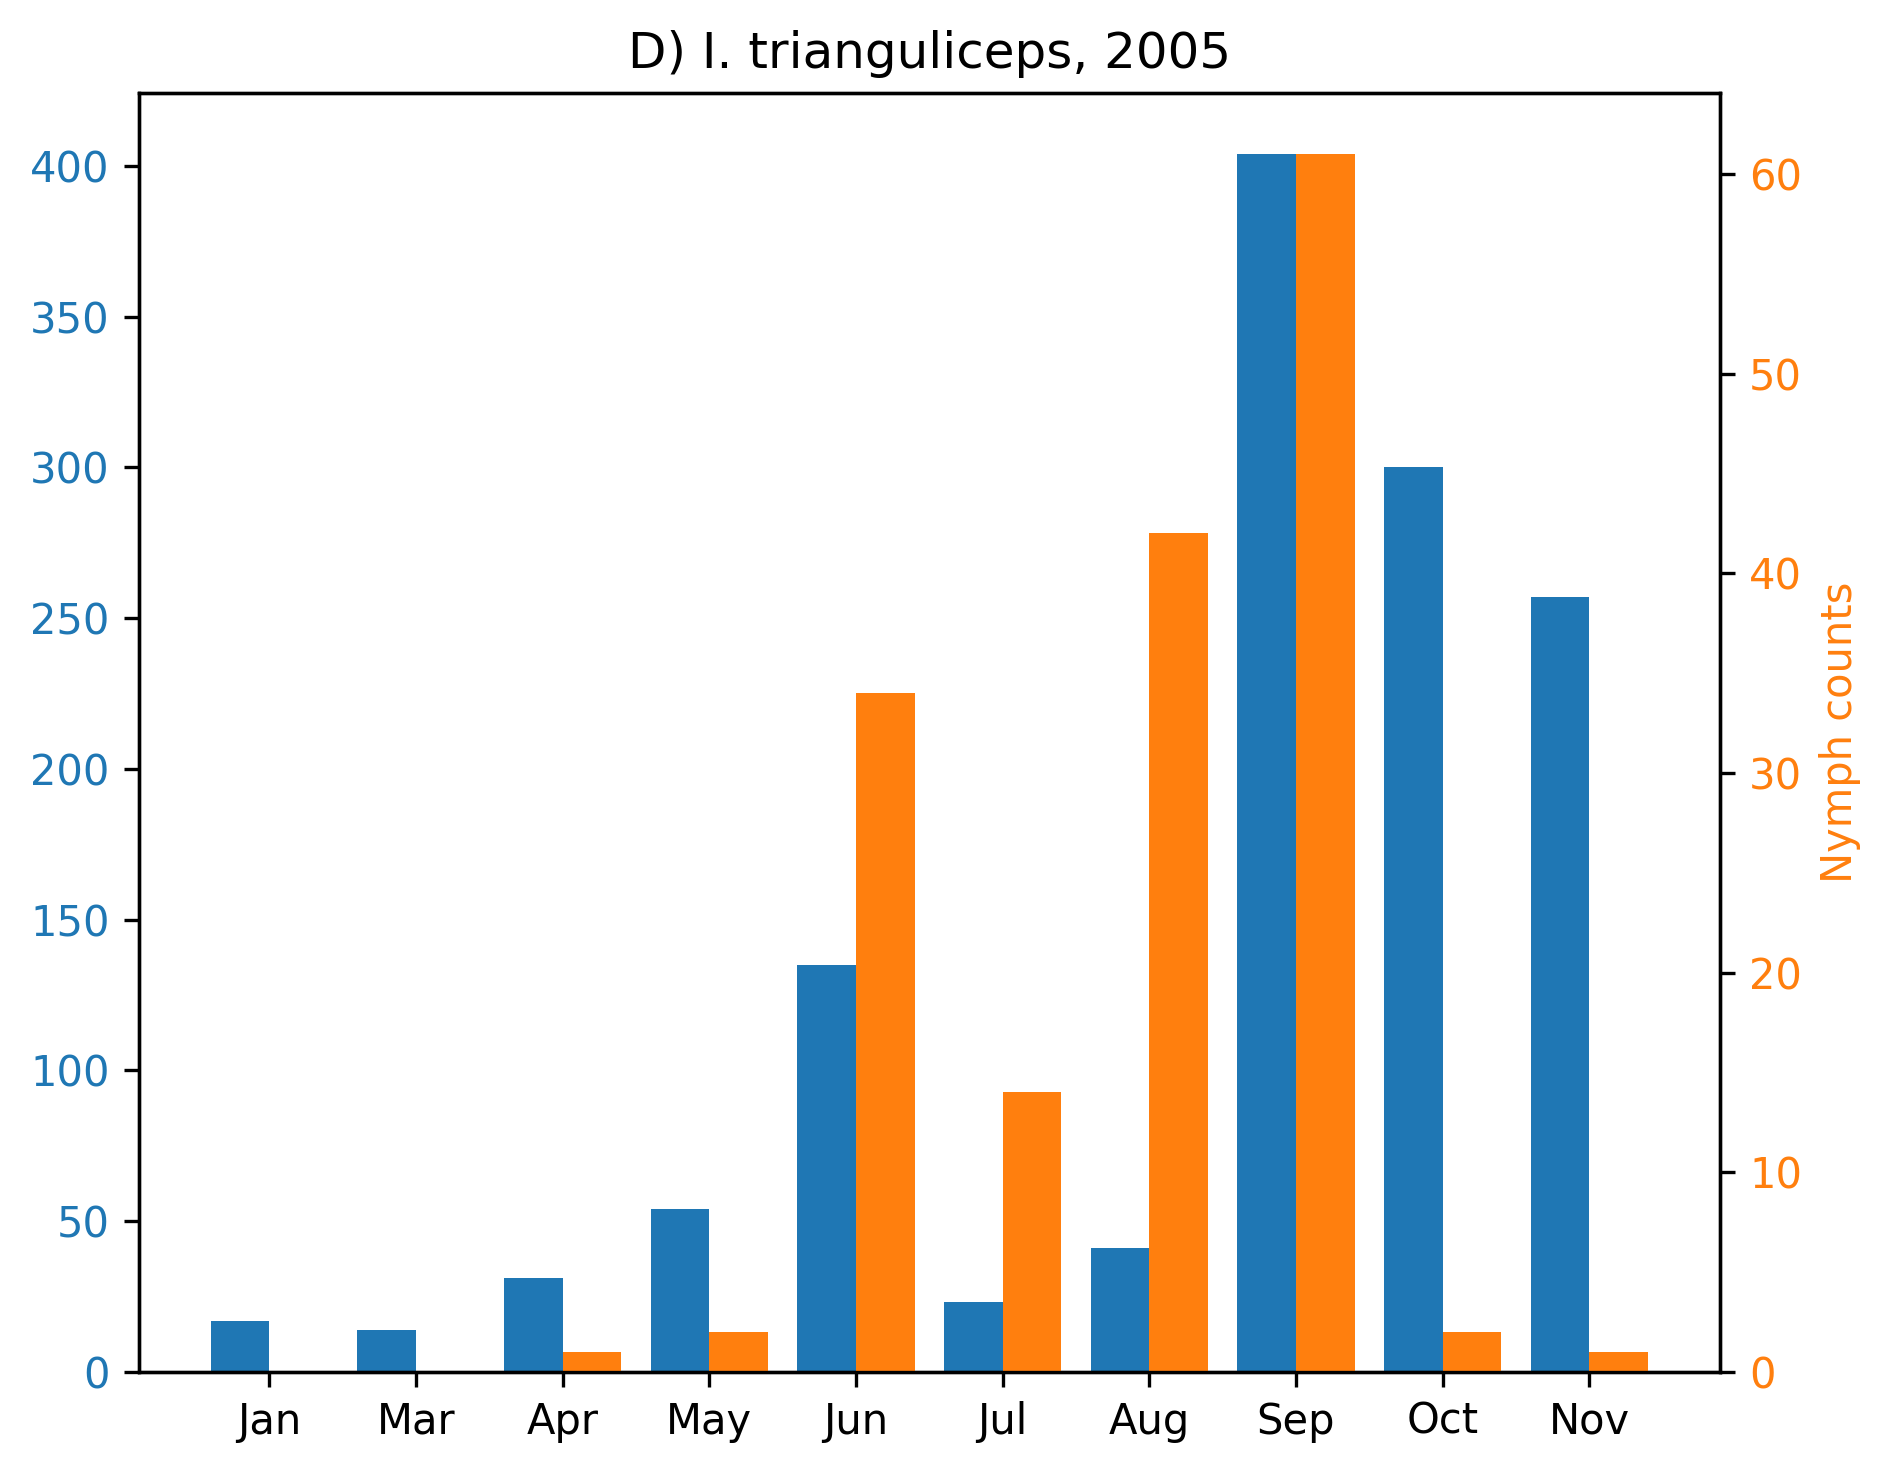
\includegraphics[width=.5\linewidth,valign=m]{D) I. trianguliceps, 2005} \\
	\end{tabular}
	\caption{ Seasonal nymphal and larval activity for \textit{I. trianguliceps} and \textit{I. ricinus} for 2004 and 2005. The data here shows the combined frequency of tick counts found on field vole and common shrew individuals.}
	\label{fig:kielder_seasonal}
\end{figure}

Overall counts of larval and nymphal burdens for both species of tick, and for the common shrew and field vole host species, are presented in table \ref{tab:counts_kielder}.

\begin{table}[h!]
	\centering
	\begin{tabular}{|llrrrr|}
		\hline
		\multicolumn{6}{|c|}{\textbf{\begin{tabular}[c]{@{}c@{}}Co-aggregation data (count data) \\ Kielder Forest\end{tabular}}}                                                                               \\ \hline
		\multicolumn{2}{|l|}{\multirow{2}{*}{}}                                         & \multicolumn{2}{c|}{\textit{I. ricinus}}                  & \multicolumn{2}{c|}{\textit{I. trianguliceps}}            \\ \cline{3-6} 
		\multicolumn{2}{|l|}{}                                                          & \multicolumn{1}{l|}{Larvae} & \multicolumn{1}{l|}{Nymphs} & \multicolumn{1}{l|}{Larvae} & \multicolumn{1}{l|}{Nymphs} \\ \hline
		\multicolumn{1}{|l|}{\multirow{2}{*}{2004}} & \multicolumn{1}{l|}{Common shrew} & \multicolumn{1}{r|}{451}    & \multicolumn{1}{r|}{14}     & \multicolumn{1}{r|}{1302}   & 137                         \\ \cline{2-6} 
		\multicolumn{1}{|l|}{}                      & \multicolumn{1}{l|}{Field vole}   & \multicolumn{1}{r|}{150}    & \multicolumn{1}{r|}{13}     & \multicolumn{1}{r|}{432}    & 4                           \\ \hline
		\multicolumn{1}{|l|}{\multirow{2}{*}{2005}} & \multicolumn{1}{l|}{Common shrew} & \multicolumn{1}{r|}{314}    & \multicolumn{1}{r|}{0}      & \multicolumn{1}{r|}{512}    & 79                          \\ \cline{2-6} 
		\multicolumn{1}{|l|}{}                      & \multicolumn{1}{l|}{Field vole}   & \multicolumn{1}{r|}{1458}   & \multicolumn{1}{r|}{24}     & \multicolumn{1}{r|}{764}    & 78                          \\ \hline
	\end{tabular}
	\caption{Overall counts of nymphs and larvae, with several vertebrate host species removed due to low counts of ticks.}
	\label{tab:counts_kielder_overall}
\end{table}

This project makes the assumption that co-feeding is the only viable route of transmission, and that co-feeding transmission is passed from infectious nymph to larvae that are in close proximity. Furthermore, if we assume \textit{I. ricinus} and \textit{I. trianguliceps} carry pathogens for which the other tick species is not susceptible, then we can refine the data to include only the larvae that co-aggregate with nymphs of the same species, as in table \ref{tab:counts_kielder_with_same_species_nymphs}. This means that larvae found on vertebrates without a nymphal burden of the same species were excluded.

%\begin{table}[h!]
%	\centering
%	\begin{tabular}{|llrrrr|}
%		\hline
%		\multicolumn{6}{|c|}{\textbf{\begin{tabular}[c]{@{}c@{}}Co-aggregation data (count data) \\ Kielder Forest\end{tabular}}}                                                                               \\ \hline
%		\multicolumn{2}{|l|}{\multirow{2}{*}{}}                                         & \multicolumn{2}{c|}{\textit{I. ricinus}}                  & \multicolumn{2}{c|}{\textit{I. trianguliceps}}            \\ \cline{3-6} 
%		\multicolumn{2}{|l|}{}                                                          & \multicolumn{1}{l|}{Larvae} & \multicolumn{1}{l|}{Nymphs} & \multicolumn{1}{l|}{Larvae} & \multicolumn{1}{l|}{Nymphs} \\ \hline
%		\multicolumn{1}{|l|}{\multirow{2}{*}{2004}} & \multicolumn{1}{l|}{Common shrew} & \multicolumn{1}{r|}{180}    & \multicolumn{1}{r|}{14}     & \multicolumn{1}{r|}{377}    & 137                         \\ \cline{2-6} 
%		\multicolumn{1}{|l|}{}                      & \multicolumn{1}{l|}{Field vole}   & \multicolumn{1}{r|}{8}     & \multicolumn{1}{r|}{13}     & \multicolumn{1}{r|}{1}     & 4                          \\ \hline
%		\multicolumn{1}{|l|}{\multirow{2}{*}{2005}} & \multicolumn{1}{l|}{Common shrew} & \multicolumn{1}{r|}{80}     & \multicolumn{1}{r|}{0}     & \multicolumn{1}{r|}{179}    & 79                          \\ \cline{2-6} 
%		\multicolumn{1}{|l|}{}                      & \multicolumn{1}{l|}{Field vole}   & \multicolumn{1}{r|}{242}    & \multicolumn{1}{r|}{24}     & \multicolumn{1}{r|}{14}     & 78                          \\ \hline
%	\end{tabular}
%	\caption{Counts of nymphs and larvae on vertebrates where one or more nymphs were found.}
%	\label{tab:counts_kielder_with_nymphs}
%\end{table}


\begin{table}[h!]
	\centering
	\begin{tabular}{|llrrrr|}
		\hline
		\multicolumn{6}{|c|}{\textbf{\begin{tabular}[c]{@{}c@{}}Co-aggregation data (count data) \\ Kielder Forest\end{tabular}}}                                                                               \\ \hline
		\multicolumn{2}{|l|}{\multirow{2}{*}{}}                                         & \multicolumn{2}{c|}{\textit{I. ricinus}}                  & \multicolumn{2}{c|}{\textit{I. trianguliceps}}            \\ \cline{3-6} 
		\multicolumn{2}{|l|}{}                                                          & \multicolumn{1}{l|}{Larvae} & \multicolumn{1}{l|}{Nymphs} & \multicolumn{1}{l|}{Larvae} & \multicolumn{1}{l|}{Nymphs} \\ \hline
		\multicolumn{1}{|l|}{\multirow{2}{*}{2004}} & \multicolumn{1}{l|}{Common shrew} & \multicolumn{1}{r|}{48}     & \multicolumn{1}{r|}{14}     & \multicolumn{1}{r|}{369}    & 137                         \\ \cline{2-6} 
		\multicolumn{1}{|l|}{}                      & \multicolumn{1}{l|}{Field vole}   & \multicolumn{1}{r|}{7}      & \multicolumn{1}{r|}{13}     & \multicolumn{1}{r|}{1}      & 4                           \\ \hline
		\multicolumn{1}{|l|}{\multirow{2}{*}{2005}} & \multicolumn{1}{l|}{Common shrew} & \multicolumn{1}{r|}{0}      & \multicolumn{1}{r|}{0}      & \multicolumn{1}{r|}{179}    & 79                          \\ \cline{2-6} 
		\multicolumn{1}{|l|}{}                      & \multicolumn{1}{l|}{Field vole}   & \multicolumn{1}{r|}{190}    & \multicolumn{1}{r|}{24}     & \multicolumn{1}{r|}{9}      & 78                          \\ \hline
	\end{tabular}
	\caption{Counts of nymphs and larvae on vertebrates, but larvae were found to co-aggregate with one or more nymphs of the same species.}
	\label{tab:counts_kielder_with_same_species_nymphs}
\end{table}

Based on low tick burden counts, we exclude several combinations but will investigate these combinations using the Kielder Forest data:
\begin{itemize}
    \item 2004: \textit{I. ricinus} found on common shrews.
    \item 2004: \textit{I. trianguliceps} found on common shrews.
    \item 2005: \textit{I. trianguliceps} found on common shrews.
    \item 2005: \textit{I. ricinus} found on field voles.
    \item 2005: \textit{I. trianguliceps} found on field voles.
\end{itemize}

There are several sensible reasons to separate these data into these 5 separate categories, rather than analysing all data together:

\begin{itemize}
    \item \textit{I. ricinus} is non-nidicolous while \textit{I. trianguliceps} is nidicolous, indicating different behaviour REF.
    \item The pathogens transmitted by each tick species are frequently not the same pathogens REF.
    \item An adult common shrew is larger than the adult field vole REF, which implies the chances of nymphs and larvae co-aggregating in close enough proximity 
    \item Yearly seasonal variation shown in figure \ref{fig:kielder_seasonal} suggests that these ticks have peak activities at different times of the year.
\end{itemize}

Central to this project is the co-incident co-aggregation of juvenile ticks on vertebrate hosts. To check the data reflected this, we used the Spearman Correlation Coefficient to test the existence of a monotonic relationship; generally, the vertebrate hosts that have more nymphs should also have more larvae. 
We used the SciPy package in Python to perform the test. We found weak evidence of correlation for some host and tick combinations. The results presented in Table \ref{tab:spearman_kielder}.

\begin{table}[h!]
	\centering
	\begin{tabular}{|lrrrr|}
		\hline
		\multicolumn{5}{|c|}{\textbf{\begin{tabular}[c]{@{}c@{}}Spearman (ranked) Correlation Analysis \\ Kielder Forest\end{tabular}}}         \\ \hline
		\multicolumn{1}{|l|}{\multirow{2}{*}{}}                                                      & \multicolumn{2}{c|}{\textit{I. ricinus}}                             & \multicolumn{2}{c|}{\textit{I. trianguliceps}}                        \\ \cline{2-5} 
		\multicolumn{1}{|l|}{}                                                                       & \multicolumn{1}{l|}{statistic}    & \multicolumn{1}{l|}{p-value} & \multicolumn{1}{l|}{statistic}     & \multicolumn{1}{l|}{p-value} \\ \hline
		\multicolumn{1}{|l|}{Common shrew}                                                           & \multicolumn{1}{r|}{0.13401} & \multicolumn{1}{r|}{$\sim$0} & \multicolumn{1}{r|}{0.24473}  & $\sim$0                      \\ \hline
		\multicolumn{1}{|l|}{Field vole}                                                             & \multicolumn{1}{r|}{0.22757} & \multicolumn{1}{r|}{$\sim$0} & \multicolumn{1}{r|}{-0.03027} & 0.10164                      \\ \hline
		\multicolumn{1}{|l|}{\begin{tabular}[c]{@{}l@{}}Common shrew \\ and field vole\end{tabular}} & \multicolumn{1}{r|}{0.19450} & \multicolumn{1}{r|}{$\sim$0} & \multicolumn{1}{r|}{0.12317}  & $\sim$0                      \\ \hline
	\end{tabular}
	\caption{The ranked correlations between nymphs and larvae, obtained by analysing the Kielder Forest data provided by Bown et al. }
	\label{tab:spearman_kielder}
\end{table}

Assuming confidence of $ 0.95 $, then the pvalue $ > 0.05 $ of \textit{I.trianguliceps} on field voles means we cannot reject the null hypothesis that there does not exist a monotonic relationship between the counts of larvae and nymphs for that combination of tick and host species. This pair of tick and vertebrate host species also has the lowest overall number of larvae, indicating low levels of co-aggregation.

AN IMPORTANT QUESTION IS, WHAT DO WE DO WITH THIS INFORMATION. DO WE NOT ANALYSE I TRIANGULICEPS ON FIELD VOLES?

\section{Reproducing the results by Lloyd-Smith et al, 2005}

Before we follow the example set by Lloyd-Smith and others, it will be useful to re-implement parts of their work. In their 2005 paper, Lloyd-Smith and others using a branching process to analyse disease transmissions \cite{LloydSmith2005}.

Figures \ref{fig:gamma(R0,R0/k)}, \ref{fig:probabilityOfExtinction}, \ref{fig:firstGenerationToReach100Offspring} are reproduced versions of the charts shared by Lloyd-Smith et al. These illustrate the effect of the individual reproductive number $ v $. A link to the code to generate these charts is shared in the appendix.

\begin{figure}[h!]
    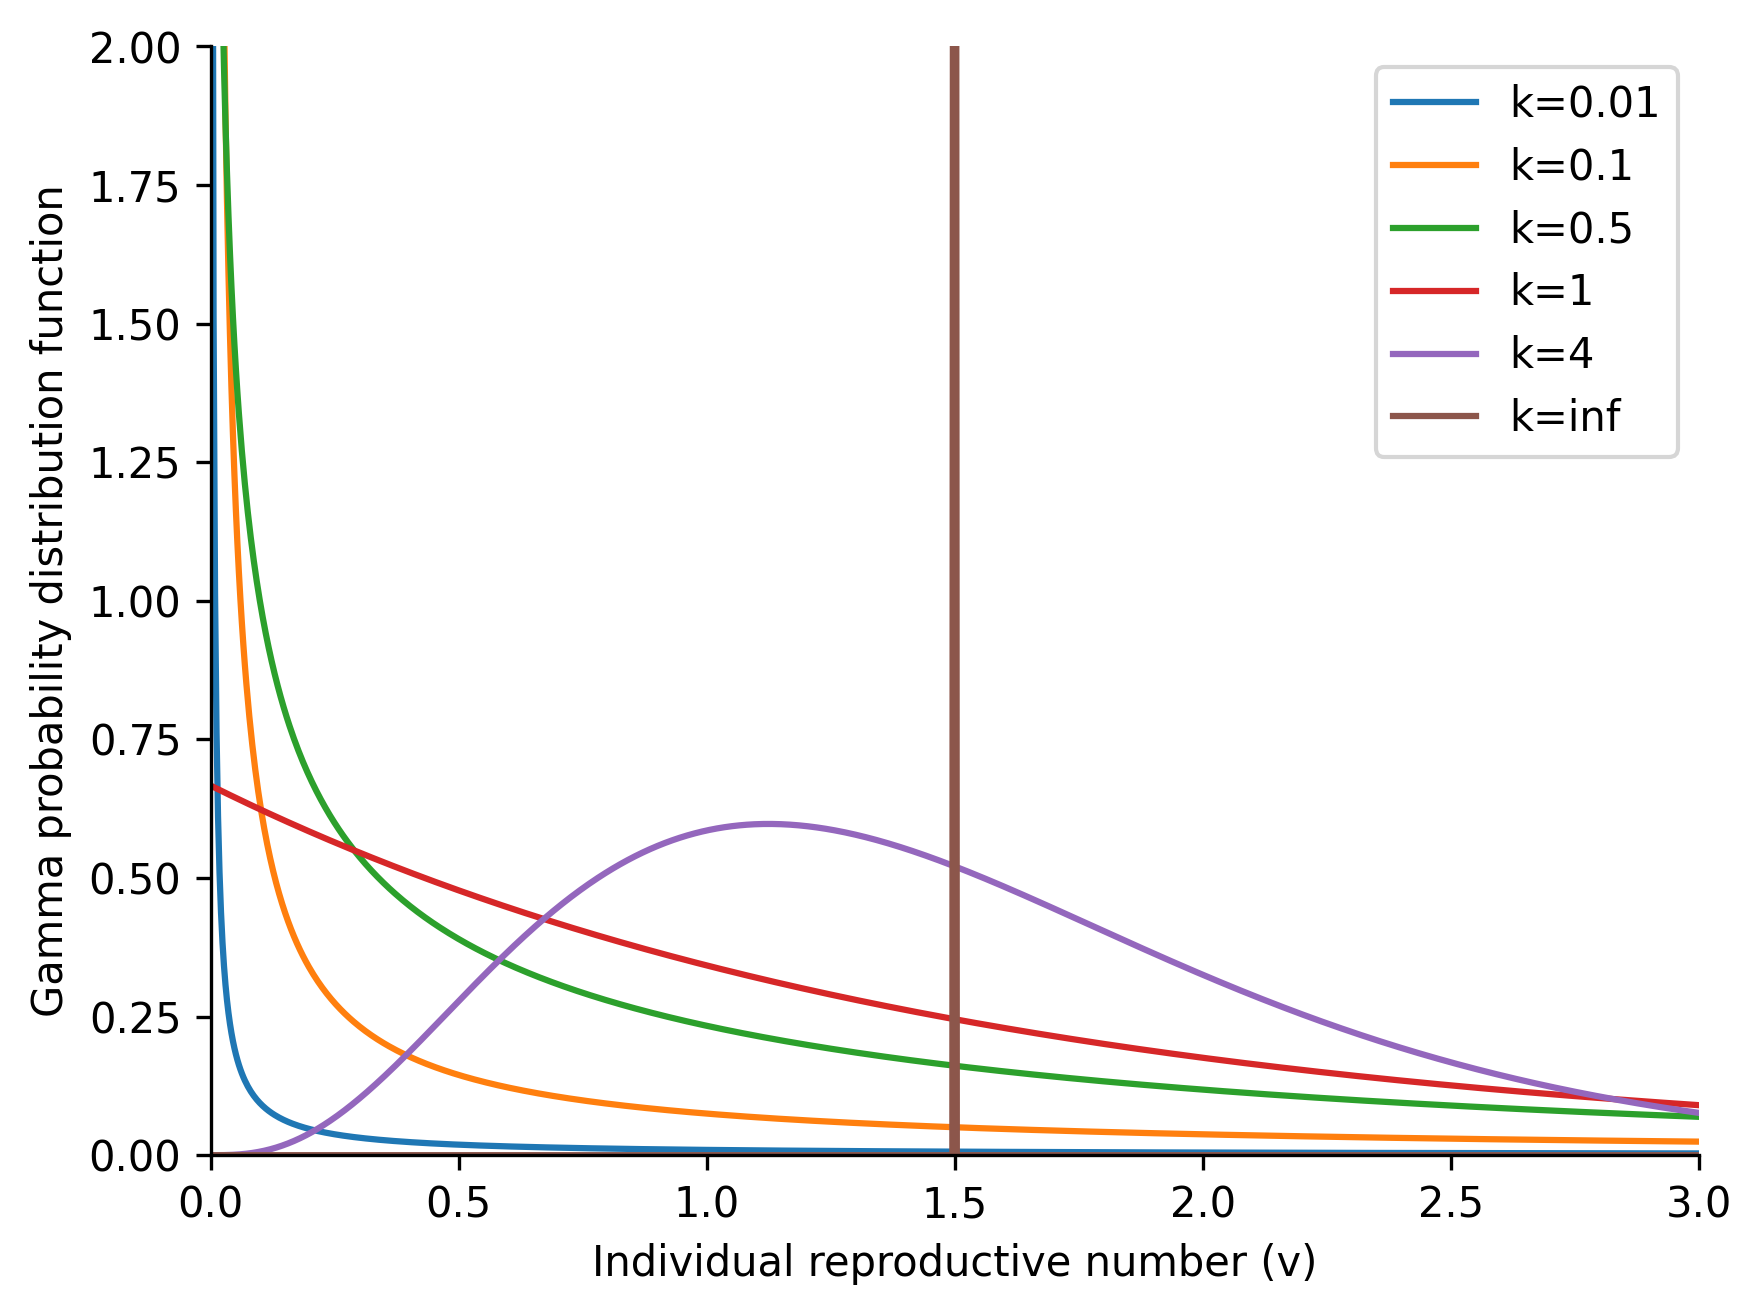
\includegraphics[width=0.5\textwidth, center]{Images/2a_gamma.png}
    \caption{The individual reproductive number $ v \sim \text{Gamma}(R_0, \frac{R_0}{k}) $. This chart shows the effect of fixing $ R_0=1.5 $ and allowing $ k $ to vary.}
    \label{fig:gamma(R0,R0/k)}
\end{figure}

\begin{figure}[h!]
    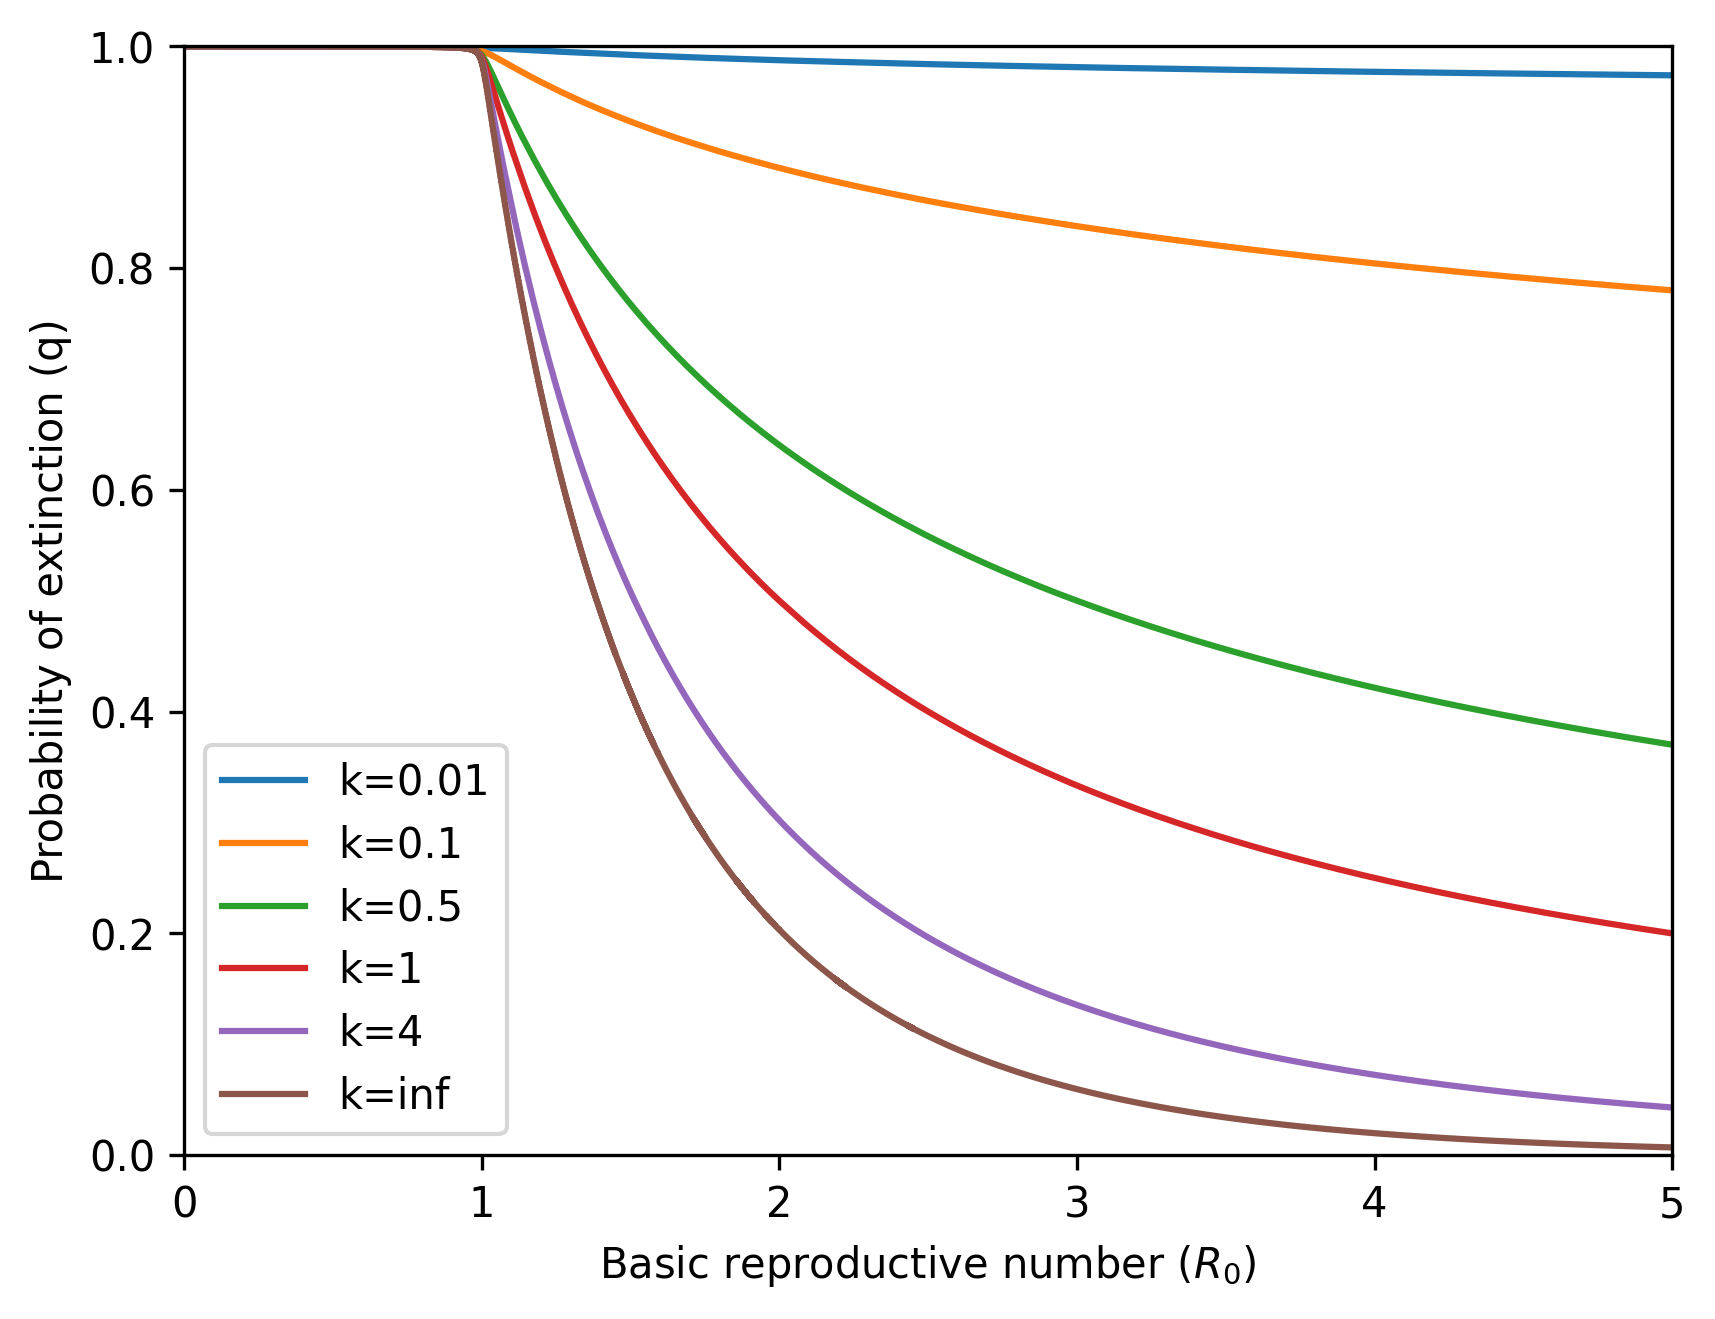
\includegraphics[width=0.5\textwidth, center]{Images/2b_probabilityOfExtinction.png}
    \caption{If $ Z \sim \text{Poisson}(v) $, then the resulting Poisson Mixture is a negative binomial distribution, which is the candidate offspring distribution. The probability that a chain of transmissions becomes extinct for a combination of $R_0$ and $ k $, after the introduction of a single infected individual, is found by fixed point iteration over the negative binomial distribution's probability generating function. Each simulation generates a random value for $ v \sim \text{Gamma}(R_0, \frac{R_0}{k})$, and these are used to generate different }\label{fig:probabilityOfExtinction}
\end{figure}

\begin{figure}[h!]
    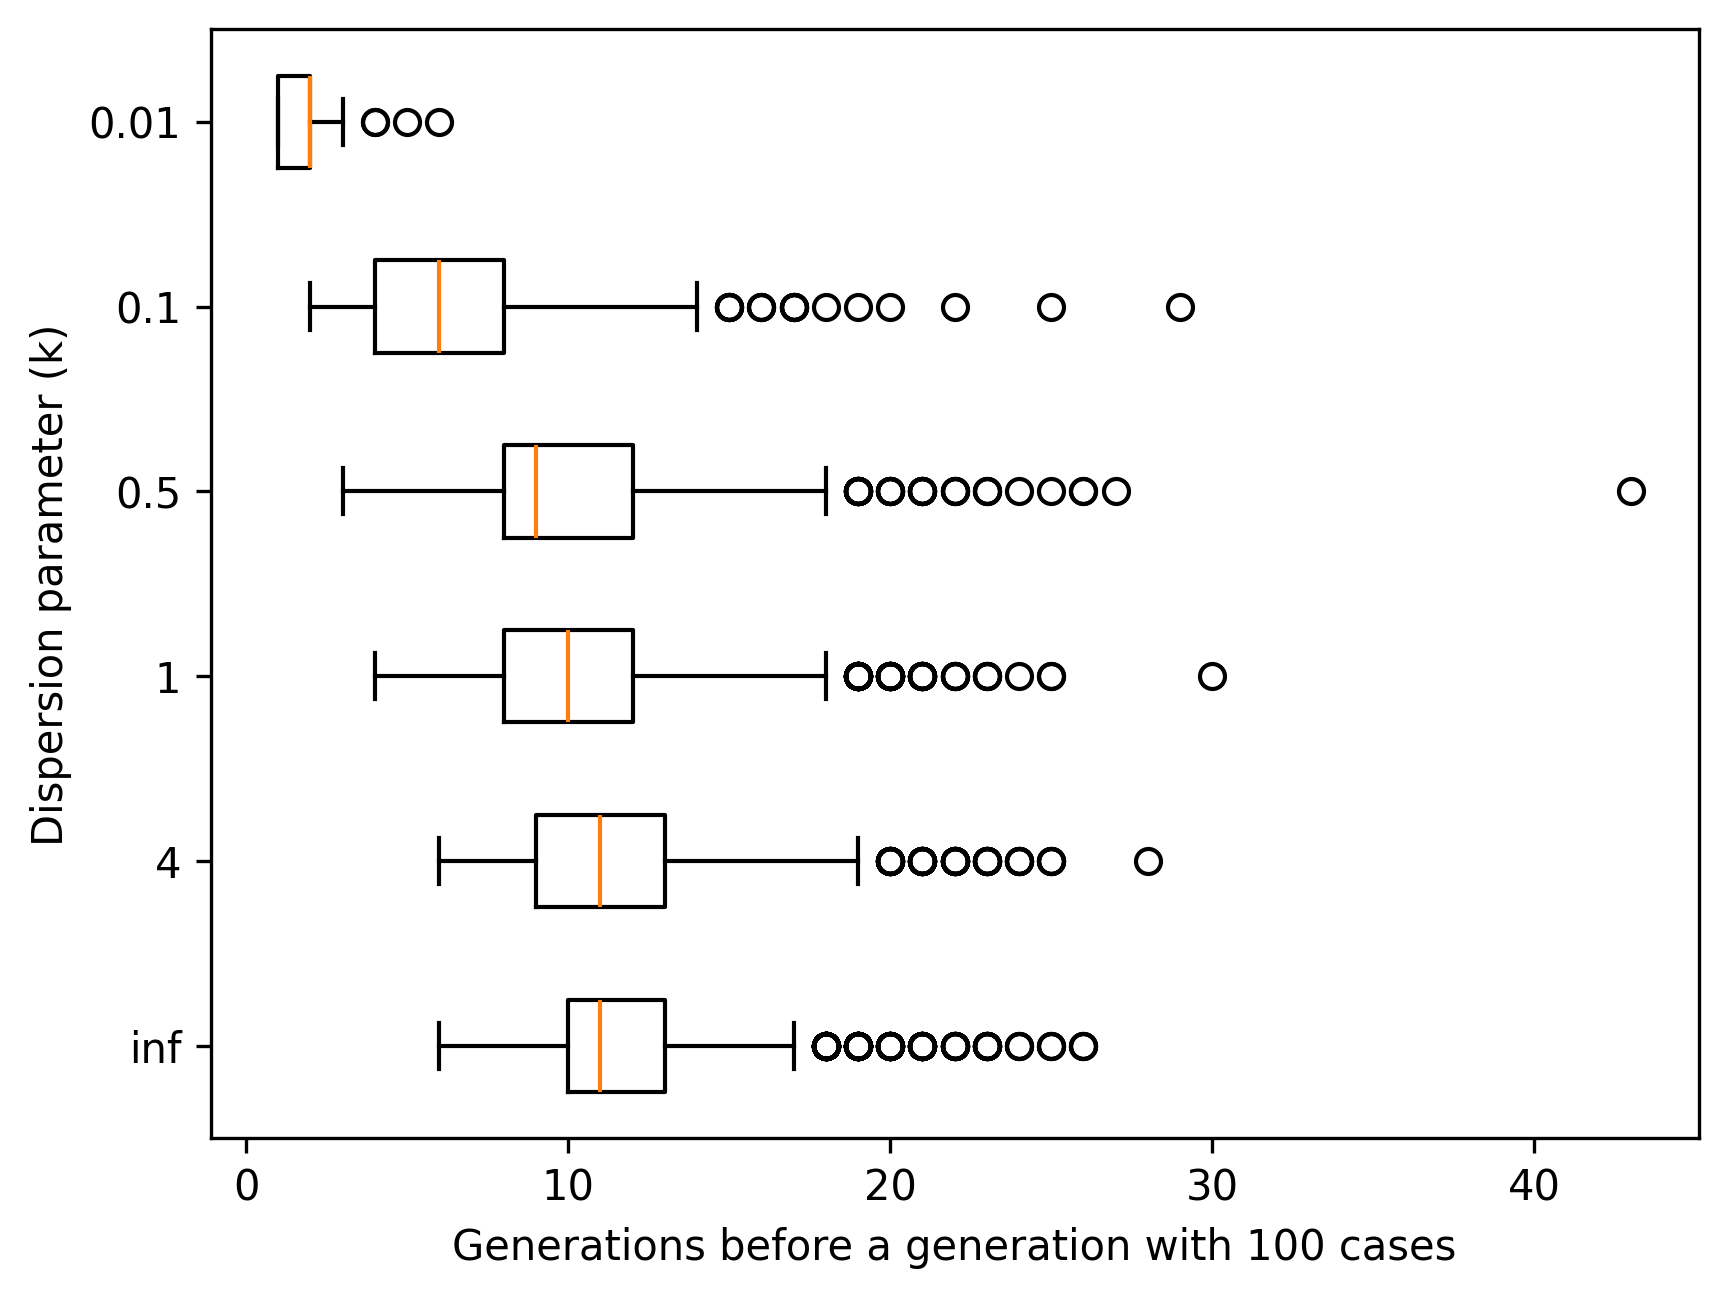
\includegraphics[width=0.5\textwidth, center]{Images/2c_firstGenerationReach100Offspring.png}
    \caption{Lloyd-Smith et al used a simulation, with the first generation to reach 100 offspring used as an arbitrary benchmark. Boxes represent the interquartile ranges for how many generations were required before a single generation contained 100 offspring, given different values of $ k $, and a fixed $ R_0=1.5 $. }\label{fig:firstGenerationToReach100Offspring}
\end{figure}

FIX THIS PARAGRAPH
Lloyd-Smith et al also showed that if $ v \sim \text{Gamma}(R_0, \frac{R_0}{k}) $, then the resulting offspring distribution is the Negative Binomial distribution. 

If we represent this as a Poisson Process, then \eqref{BranchingProcess} becomes:

\begin{equation}
    g(s) = \displaystyle \int_{0}^{\infty} e^{-u(1-s)} f_v(u) du
\end{equation}

And, if $ v \sim \text{Gamma}(R_0, \frac{R_0}{k}) $ then (2) becomes:

\begin{equation}
    g(s) = \left( 1 + \frac{R_0}{k}(1-s) \right)^{-1}
\end{equation}

Then, if we wish to calculate the probability that a chain of transmissions becomes extinct at or before generation $ m $, then we can use (3) as a recurrence relation:

\begin{align}
    q_{m+1} = g(q_{m}) &= \left( 1 + \frac{R_0}{k}(1-q_{m}) \right)^{-1} \\
    q = g(q) &= \left( 1 + \frac{R_0}{k}(1-q) \right)^{-1}
\end{align}

The equation (EQ) simplifies to (EQ), because all $ q_m \le 1 $ and $ q_{m+1} \ge q_m $, meaning the series monotonically increases to a finite value. In other words, it converges.

Then $q = g(q) $, which is a function that is equal to its independent variable, which is known as a fixed point. We can approximate the value, via Fixed Point Iteration, to some acceptable measure of error.

This result, with Fixed Point Iteration, we will use later to estimate the probability that a chain of co-feeding transmissions becomes extinct.

\section{A model of co-feeding in a TBD network}

WRITE DETAILS OF OUR MODEL OF BIOLOGICAL REALITY, BASED ON GRAPHICAL ABSTRACT

\section{Parameterisation of the Negative Binomial distribution}

A candidate for the offspring distribution is the negative binomial distribution. Other candidate discrete distributions are the Poisson and geometric distributions; later in this project, we fit all distributions to the same data and then compare goodness-of-fit. 

Commonly, the negative binomial distribution uses the number of successes or failures and the probability of success for the shape parameters. But, a more convenient parameterisation uses the sample mean $ m $ and dispersion parameter $ k $ as parameters \cite{Rice2007}:

\begin{equation}\label{NegBinomReparam}
    Z \sim NB(x | m, k) = \left(1+\frac{m}{k}\right)^{-k} \space \frac{\Gamma(k+x)}{x!\Gamma(k)} \space \left(\frac{m}{m+k}\right)^x, \space \space \space \space \space x \in \mathbb{N}
\end{equation}

Finding $ R_0 $ by analysing contact-trace data also determines $ m $ for this distribution, by setting $ m=R_0 $. Finding the dispersion parameter $ k $ is achievable with maximum likelihood estimation (MLE). Since the parameters are asymptotically orthogonal \cite{LloydSmith2005}, then we can find $ k $ via MLE without doing so for $ m $.

In this project, we tested the standard negative binomial distribution, available in Python Scipy, against the reparameterisation (\ref{NegBinomReparam}) by fitting both distributions to the same data. Results indicate a similar fit. A link to the code is available in the appendix.

\section{The probability that a chain of TBD transmissions becomes extinct}

Given the scenario where a single infected tick is introduced to a population of vertebrate hosts for the first time, there is no guarantee that the tick will infect any other tick. Even if it did, those infected ticks might not infect any others for a number of reasons. There is no reason to think that all ticks will share the same individual reproductive number $ v $. Deterministic systems of equations, and their underlying assumption of homogeneity, are not appropriate for estimating the probability that a chain of transmissions in a TBD network becomes extinct in the first stages of an outbreak.

To calculate the probability that a chain of TBD transmissions becomes extinct, we can use a GWBP analysis similar to the example set by Lloyd-Smith and others used in their 2005 paper \cite{LloydSmith2005}. To do that, however, we first require a candidate for the offspring distribution.

\subsection{Finding a candidate offspring distribution}

Lloyd-Smith and others estimated $ R_0 $ and then found an estimate for $ k $ by using contact-tracing network data, ??AND COUNTING ZEROS??. In our case, we have empirical data for the co-aggregation of larvae and nymphs, but this does not mean that each pair of larva and nymph was a transmission. We could use a stochastic process simulate a transmission network based on the empirical data. 

Let us note some characteristics of diseases where \textit{Ixodidae} tick species are the vectors:
\begin{itemize}
	\item Since a larva will take one blood meal before it moults into a nymph, then the only way for an \textit{Ixodidae} larva to be infectious when it takes its blood meal would be if it was already infected via transovarial transmission.
	\item Given that ticks die during and between their life stages, then larvae will be relatively common, nymphs less common, and adults less common still \cite{Randolph1998}.
	\item Adult ticks tend to feed on larger vertebrates, whereas immature ticks (larvae and nymphs) frequently feed on small vertebrate hosts \cite{Herrmann2015, Randolph1998}.
	\item Since immature ticks prefer to feed on smaller vertebrate hosts, then they are more likely to feed in close proximity.
	\item Nymph-to-nymph co-feeding transmission is rare \cite{VOORDOUW2014}.
\end{itemize}

So, if a TBD was to spread through a population of ticks via co-feeding only, in the absence of transovarial and systemic transmission, then the majority of infections would pass from nymphs to larvae. Each larva would need to moult into a nymph and then successfully find another host before it could then pass the pathogen onto larvae that it co-aggregates with. During moulting the pathogen would need to survive transstadially as each infected larva becomes an infectious nymph. The ticks that co-aggregate would need to feed close enough for the transmission to occur.

Then, let us introduce these terms:

\begin{description}[leftmargin=1cm, style=nextline]
    \item[$ c $] be the contact rate, or the probability that a larva and infectious nymph co-aggregate close enough for transmission to occur.
    \item[$ v $] be the probability of transmission, since individual variation means not every infectious nymph has the same capability to transmit the disease.
    \item[$ \sigma $] be the probability that a larvae survives to become a nymph (moulting success).
    \item[$ \tau $] be the probability that transstadial transmission occurs.
\end{description}

Then for each larvae that co-aggregates with an infectious nymph, the probability that it becomes an infectious nymph is found by:

\begin{equation} \label{alphaDef}
    \alpha = c v \sigma \tau
\end{equation}

$ \alpha $ will depend on the species of tick, the pathogen being transmitted, the vertebrate host ticks feed on, seasonal variation and perhaps other factors.

The network thinking by Johnstone-Robertson et al, in their 2020 paper \cite{JohnstoneRobertson2020}, is important for this project. Their superimposition of tick-to-tick transmission onto the tick-host contact network is the inspiration for this idea: we can use co-aggregation data to generate a nymph-larvae contact network for each nymph.

Then let:
\begin{description}[leftmargin=1cm, style=nextline]
    \item[$ X $] be a vector of the out degree for each nymph's larval contact network.
    \item[$ X_\alpha $] be a vector for how many larvae become infectious nymphs. This is offspring data to which we will fit a distribution, as the offspring distribution. Note that $ X $ and $ X_\alpha $ have the same number of elements. 
\end{description}

Conceptually, we could fit a probability distribution to $ X $ and then draw random values from that, then apply the stochastic process using $ \alpha $ to find $ X_\alpha $, to then fit a probability  distribution to it as the offspring distribution. That would be everything that we need to use the GWBP approach to numerically determine the probability that a chain of transmissions becomes extinct. However, we can avoid the stochastic simulation, as shown  later in this thesis.

\begin{figure}[h!]
    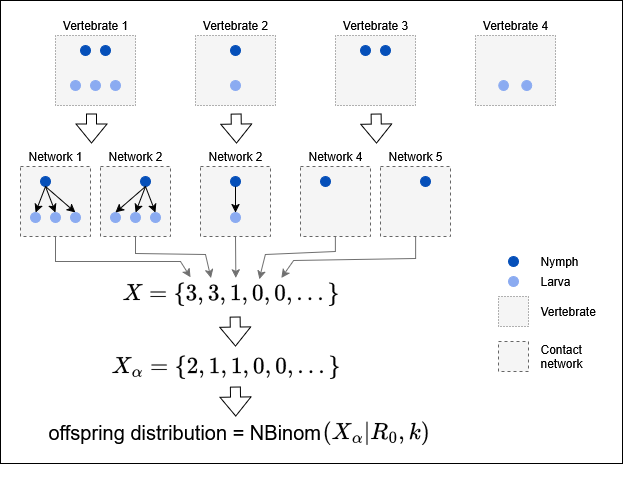
\includegraphics[width=1\textwidth, center]{Images/coaggregation_data_diagram_mk3.drawio.png}
    \caption{A toy example of how we find the offspring distribution. Each nymph has its own contact network with larvae. The out degree for each nymph is the number of larvae that it coaggregates with. A stochastic step is applied to the vector $ X $ to determine the number of larvae that become infectious nymphs. $ R_0 $ and $ k $ are then found by fitting the reparameterised negative binomial distribution to $ X_\alpha $.}\label{fig:coaggregation_diagram}
\end{figure}

\subsection{Fitting a distribution to \texorpdfstring{$ X_\alpha $}{X_alpha}}

Before proceeding, we can find a probability distribution that is a good fit to the co-aggregation data $ X $, and then the offspring data $ X_\alpha $. Several discrete distributions could be the best choice: geometric, Poisson and negative binomial distributions could all fit. The negative binomial distribution is often a good fit to parasite aggregation data, and, Lloyd-Smith and others showed this was the best fit for several disease transmission networks; we can expect that the negative binomial distribution will be the best fit. The following assumes that the reparameterised negative binomial distribution is an appropriate fit to $ X $. Later, we test its goodness-of-fit against the Poisson and geometric distributions.

Let:

\begin{description}[leftmargin=1cm, style=nextline]
	\item[$ n $] be the number of nymphs in the analysis, also the length of $ X $
	\item[$ k $] be the dispersion parameter.
	\item [$ m = \frac{1}{n} \sum_i^n L_i $] be the mean of $ X $.
	\item [$ L_i \sim \text{NB}(X | m, k) $] be the co-aggregation distribution, fit to $ X $. This is the reparameterised negative binomial distribution (\ref{NegBinomReparam}).
	$ L_i $ is the number of larvae that co-aggregate with a nymph of index $ i $.
	\item [$ I_{i,j} \sim \text{Bern}(p=\alpha) $] be a Bernoulli trial, or, a coin flip for each nymph of index $ i $ and for each larvae that it co-aggregates with, indexed by $ j \in 1:L_i $. This is a step where an infectious nymph generates a new infectious nymph, which is an offspring in the GWBP.
	\item [$ R_0 $] be the basic reproductive number. This is also the mean value of the offspring data $ X_\alpha $
	\item [$ Z \sim \text{NB}(X_\alpha|m=R_0, k) $] be the offspring distribution. This is achieved by  simulating offspring data $ X_\alpha $ and then fitting the distribution to it. This will have mean $ R_0 $.
\end{description}

To get the expected number of new infectious nymphs per current infectious nymph, dependent on the number of larvae that each infectious nymph co-aggregates with, the number of new infections is a series of Bernoulli trials, where $ L_i $ is the number of trials. This is otherwise known as a binomial experiment:

\begin{align}
    I_i &= \sum_j^{L_i} I_{i,j} \nonumber \\
    I_i &\sim \text{Binom}(L_i,\alpha)\label{BinomialExperiment}
\end{align}

The expected value of the binomial distribution in \eqref{BinomialExperiment} is $ \mu_i = L_i \alpha $, which is the expected number of new infections for the nymph of index $ i $.

Then to determine $ R_0 $, which is the expected number of new infections in an offspring distribution, this is:

\begin{align}\label{FindingR0FromCoaggregationMean}
    R_0 &= \frac{1}{n} \sum_i^n \mu_i \nonumber \\
    R_0 &= \frac{1}{n} \sum_i^n L_i \alpha \nonumber \\
    R_0 &= \alpha \frac{1}{n} \sum_i^n L_i \nonumber \\
    R_0 &= \alpha m
\end{align}

In summary, by fitting the co-aggregation distribution to $ X $, we can find the mean parameter for the $ X_\alpha $ by scaling the $ X $ mean value by $ \alpha $. This allows us to avoid using computation to determine which larvae become infectious nymphs.

\subsection{Estimates for \texorpdfstring{$ \alpha $}{alpha}}

Before fitting distributions to subsets of data, we should define values of $ \alpha $ defined previously (\eqref{alphaDef}). These estimates will be illustrative, but researchers who wish to calculate the probability that a new outbreak becomes extinct will likely need to provide better estimates to learn more about their particular tick species, host species and environmental conditions.

\begin{table}[h!]
	\begin{tabular}{|lrl|}
		\hline
		\multicolumn{1}{|l|}{Parameter}  & \multicolumn{1}{l|}{Estimate} & Reason
		\\ \hline
		\multicolumn{1}{|l|}{$ c $}      & \multicolumn{1}{r|}{0.4}      & \begin{tabular}[c]{@{}l@{}}Ticks tend to feed on or near ears GET REF. Most vertebrates \\have two ears, but some vertebrates will attach away from an ear.\end{tabular} \\ \hline
		\multicolumn{1}{|l|}{$ v $}      & \multicolumn{1}{r|}{0.95}     & Arbitrarily set to be not perfect. 
		\\ \hline
		\multicolumn{1}{|l|}{$ \sigma $} & \multicolumn{1}{r|}{$ 0.5$ }      & Estimates range between $ 0.1 $ and $ 0.9 $.
		\\ \hline
	\end{tabular}
	\caption{$\alpha$ estimates for Kielder Forest data.}
	\label{table:kielderForestParamEstimates}
\end{table}

Then, for the analysis presented in the results section, $ \alpha = cv\sigma = 0.19 $

\subsection{Goodness of fit tests for co-aggregation distribution}

Before using the reparameterised negative binomial distribution (\ref{NegBinomReparam}) for determining the probability of extinction with a GWBP, we can check which distribution fits the co-aggregation data $ X $ best. Candidate distributions are the negative binomial, Poisson and geometric distributions. We compared the fitted distributions visually, and by using the Akaike Information Criterion (AIC) \cite{LloydSmith2005}.

For the visual analysis, we calculated the error of each fitted distribution by finding the difference between its cumulative density function and the data's empirical cumulative density function. We plotted this error for each subset of the Kielder Forest data. These are presented in the results section, in figures: .... 

\begin{figure}[h!]
	\centering
	\begin{tabular}{ll}
		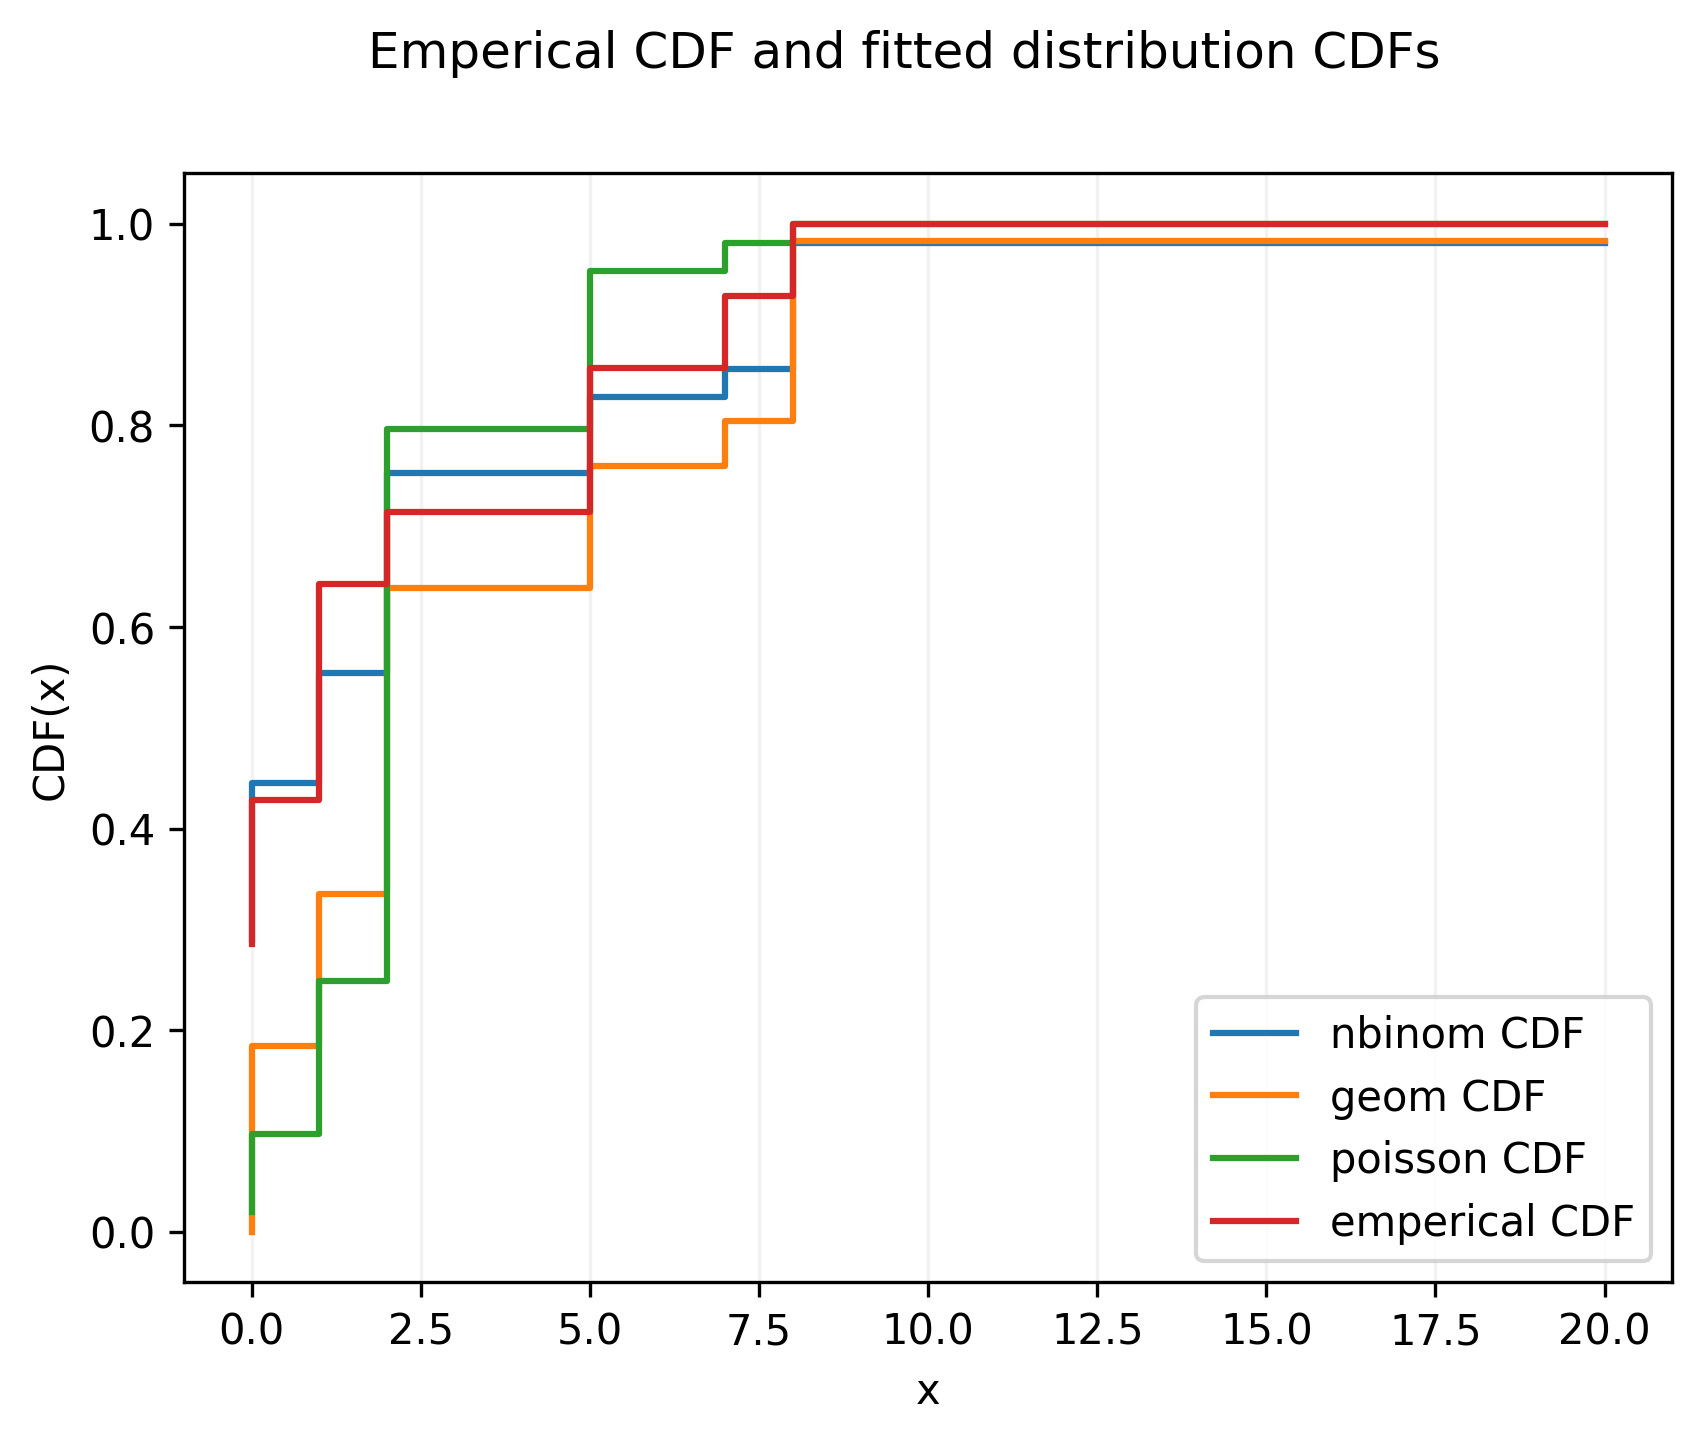
\includegraphics[width=.48\linewidth,valign=m]{CDF_compare_2004_I.ricinus_SA} & 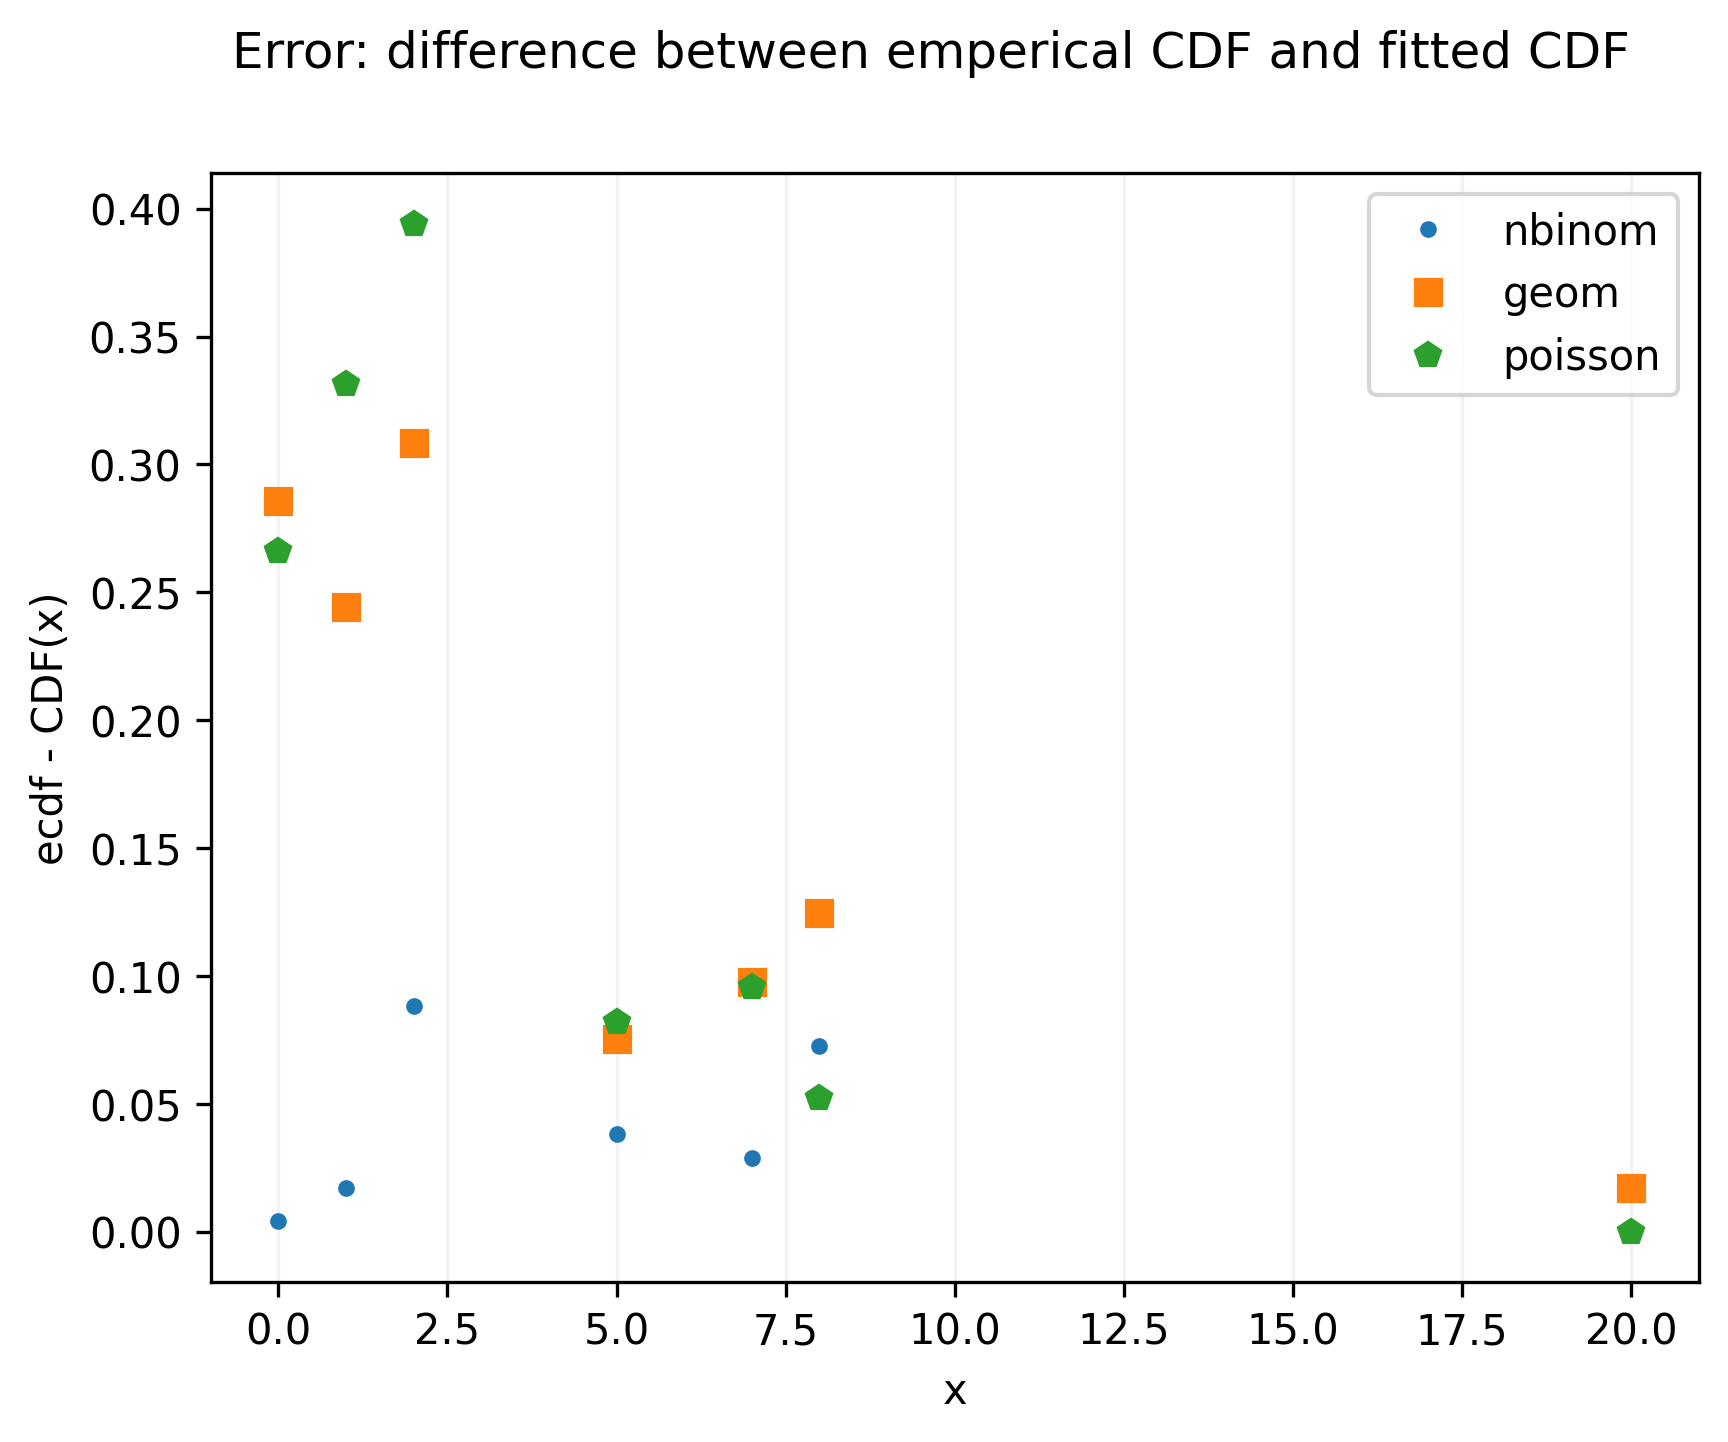
\includegraphics[width=.48\linewidth,valign=m]{CDF_errors_2004_I.ricinus_SA}
	\end{tabular}
	\caption{Discrete probability distributions fitted to the co-aggregation data $ X $ for \textit{I. ricinus} found on \textit{common shrews} in \textit{2004}.}
	\label{fig:kielder_2004_iricinus_SA}
\end{figure}

\begin{figure}[h!]
	\centering
	\begin{tabular}{ll}
		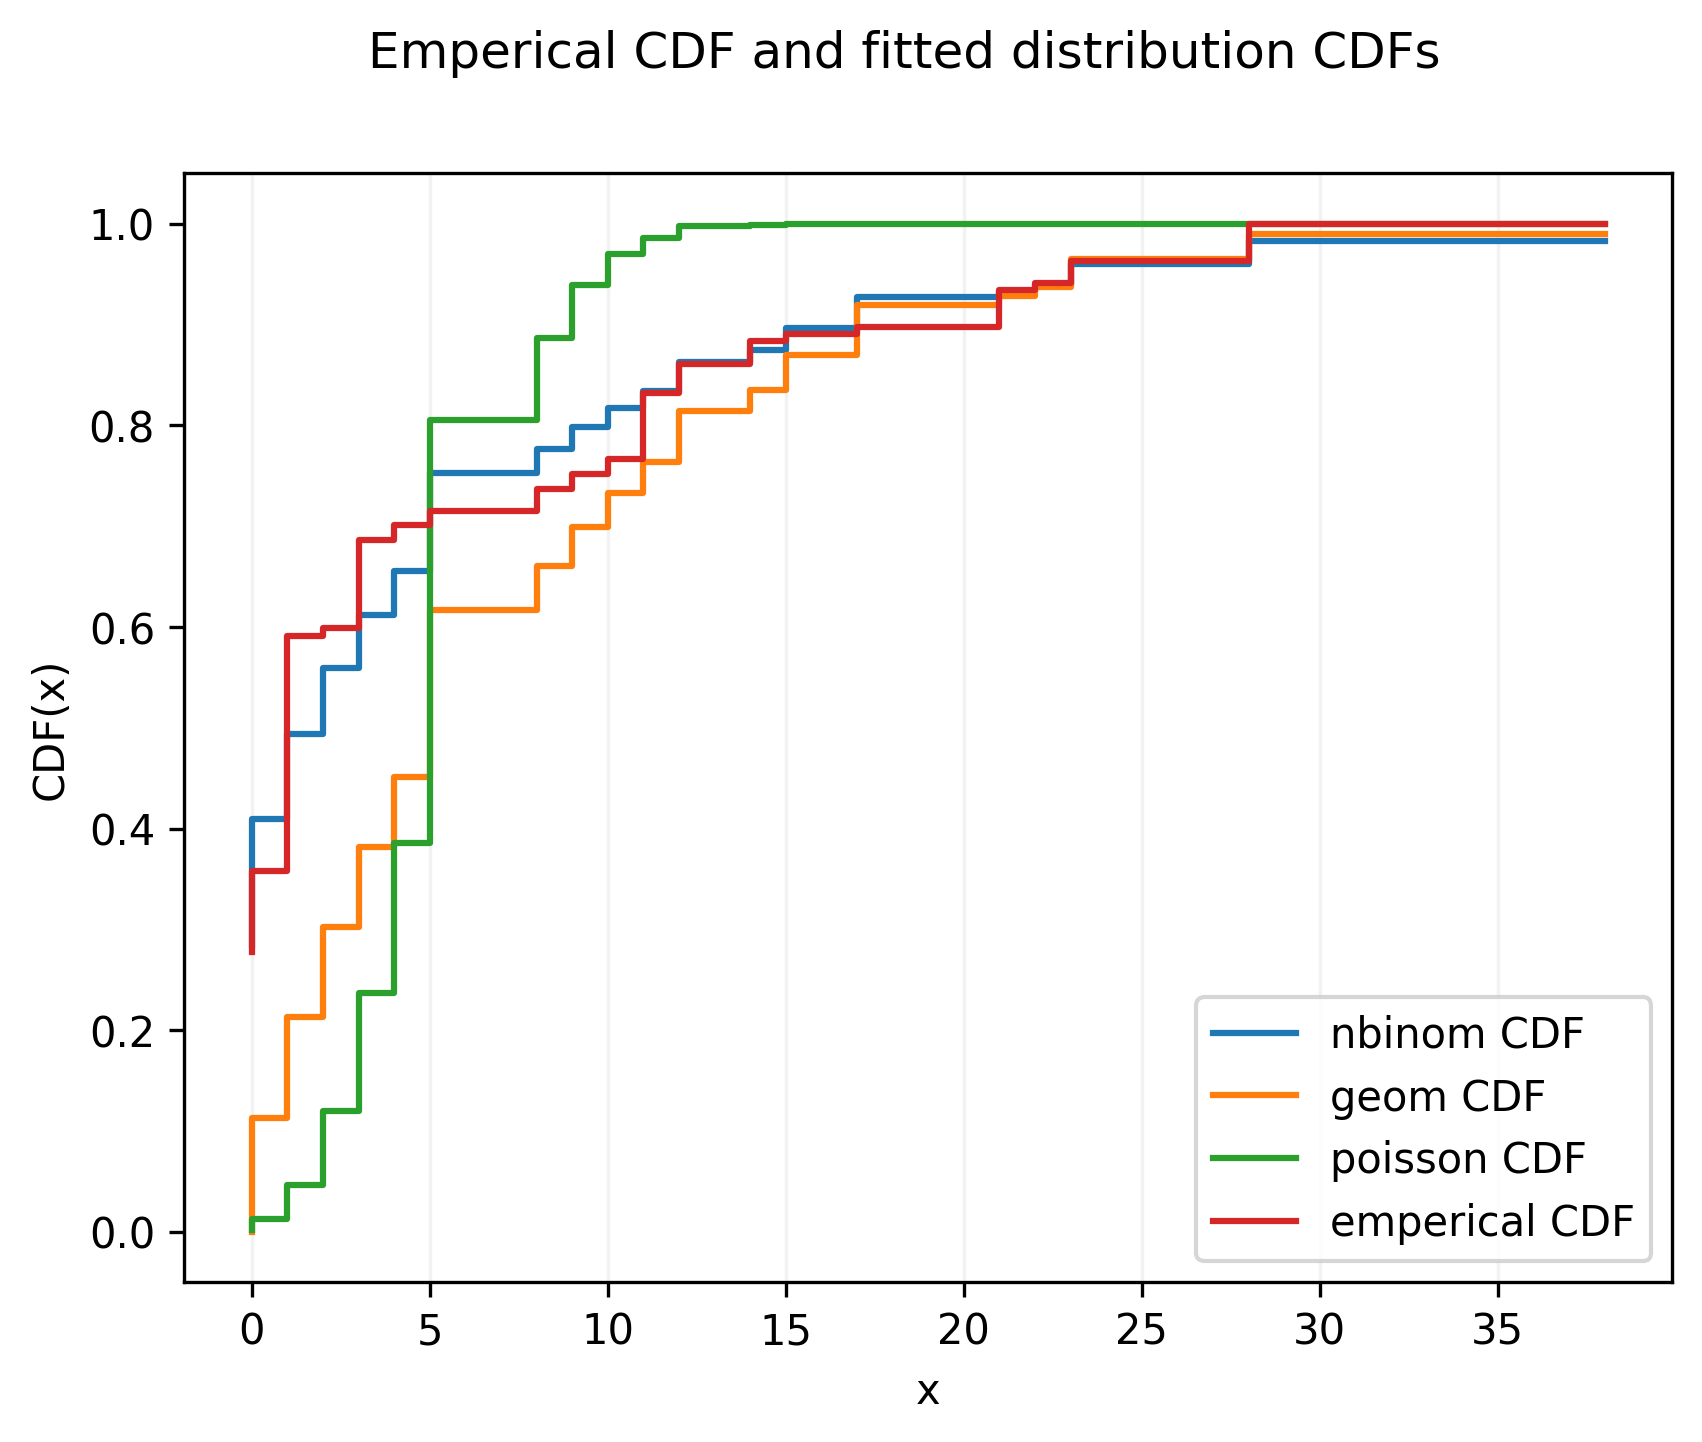
\includegraphics[width=.48\linewidth,valign=m]{CDF_compare_2004_I.trianguliceps_SA} & 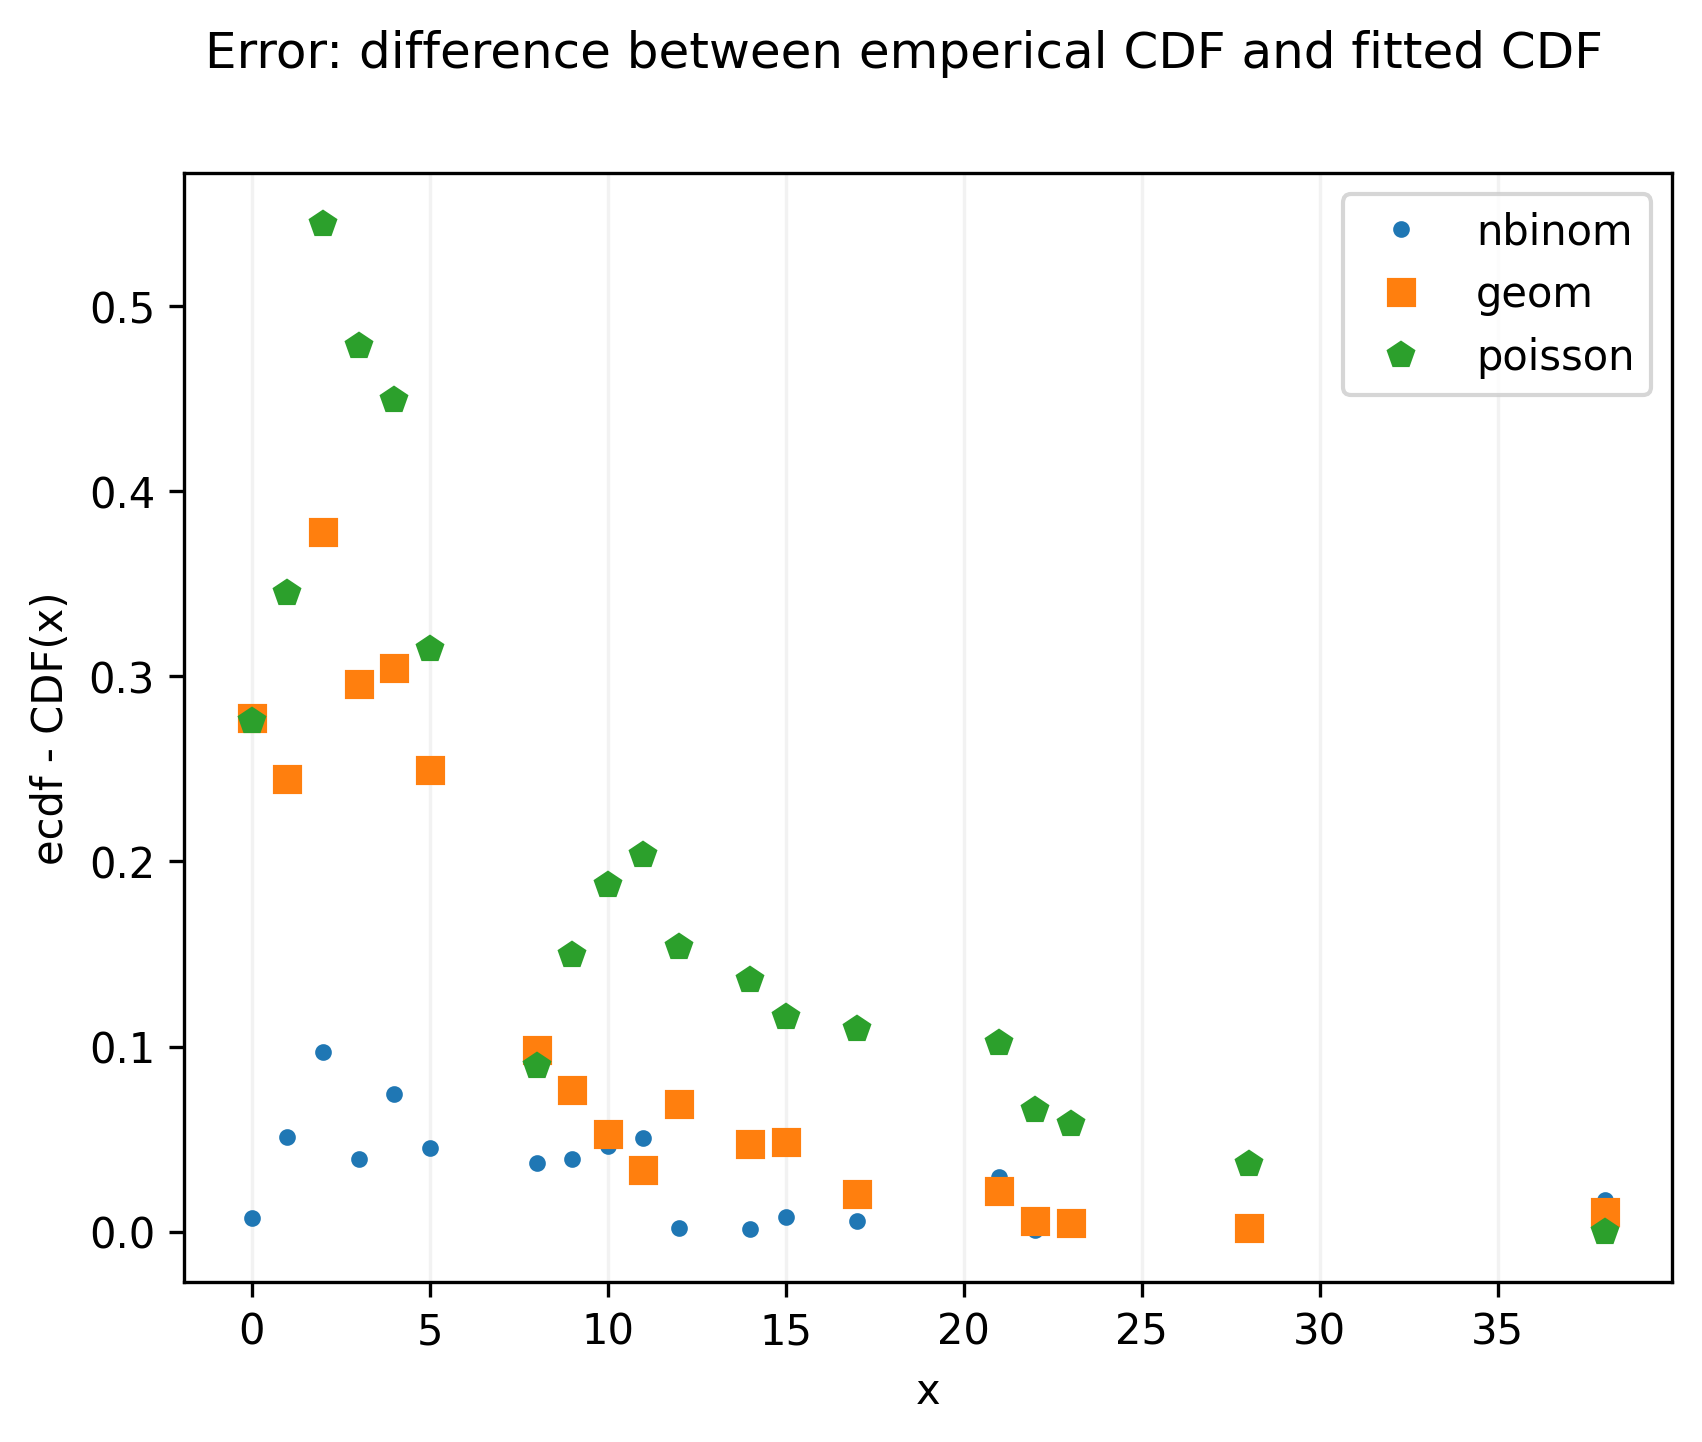
\includegraphics[width=.48\linewidth,valign=m]{CDF_errors_2004_I.trianguliceps_SA}
	\end{tabular}
	\caption{Discrete probability distributions fitted to the co-aggregation data $ X $ for \textit{I. trianguliceps} found on \textit{common shrews} in \textit{2004}.}
	\label{fig:kielder_2004_itrianguliceps_SA}
\end{figure}

\begin{figure}[h!]
	\centering
	\begin{tabular}{ll}
		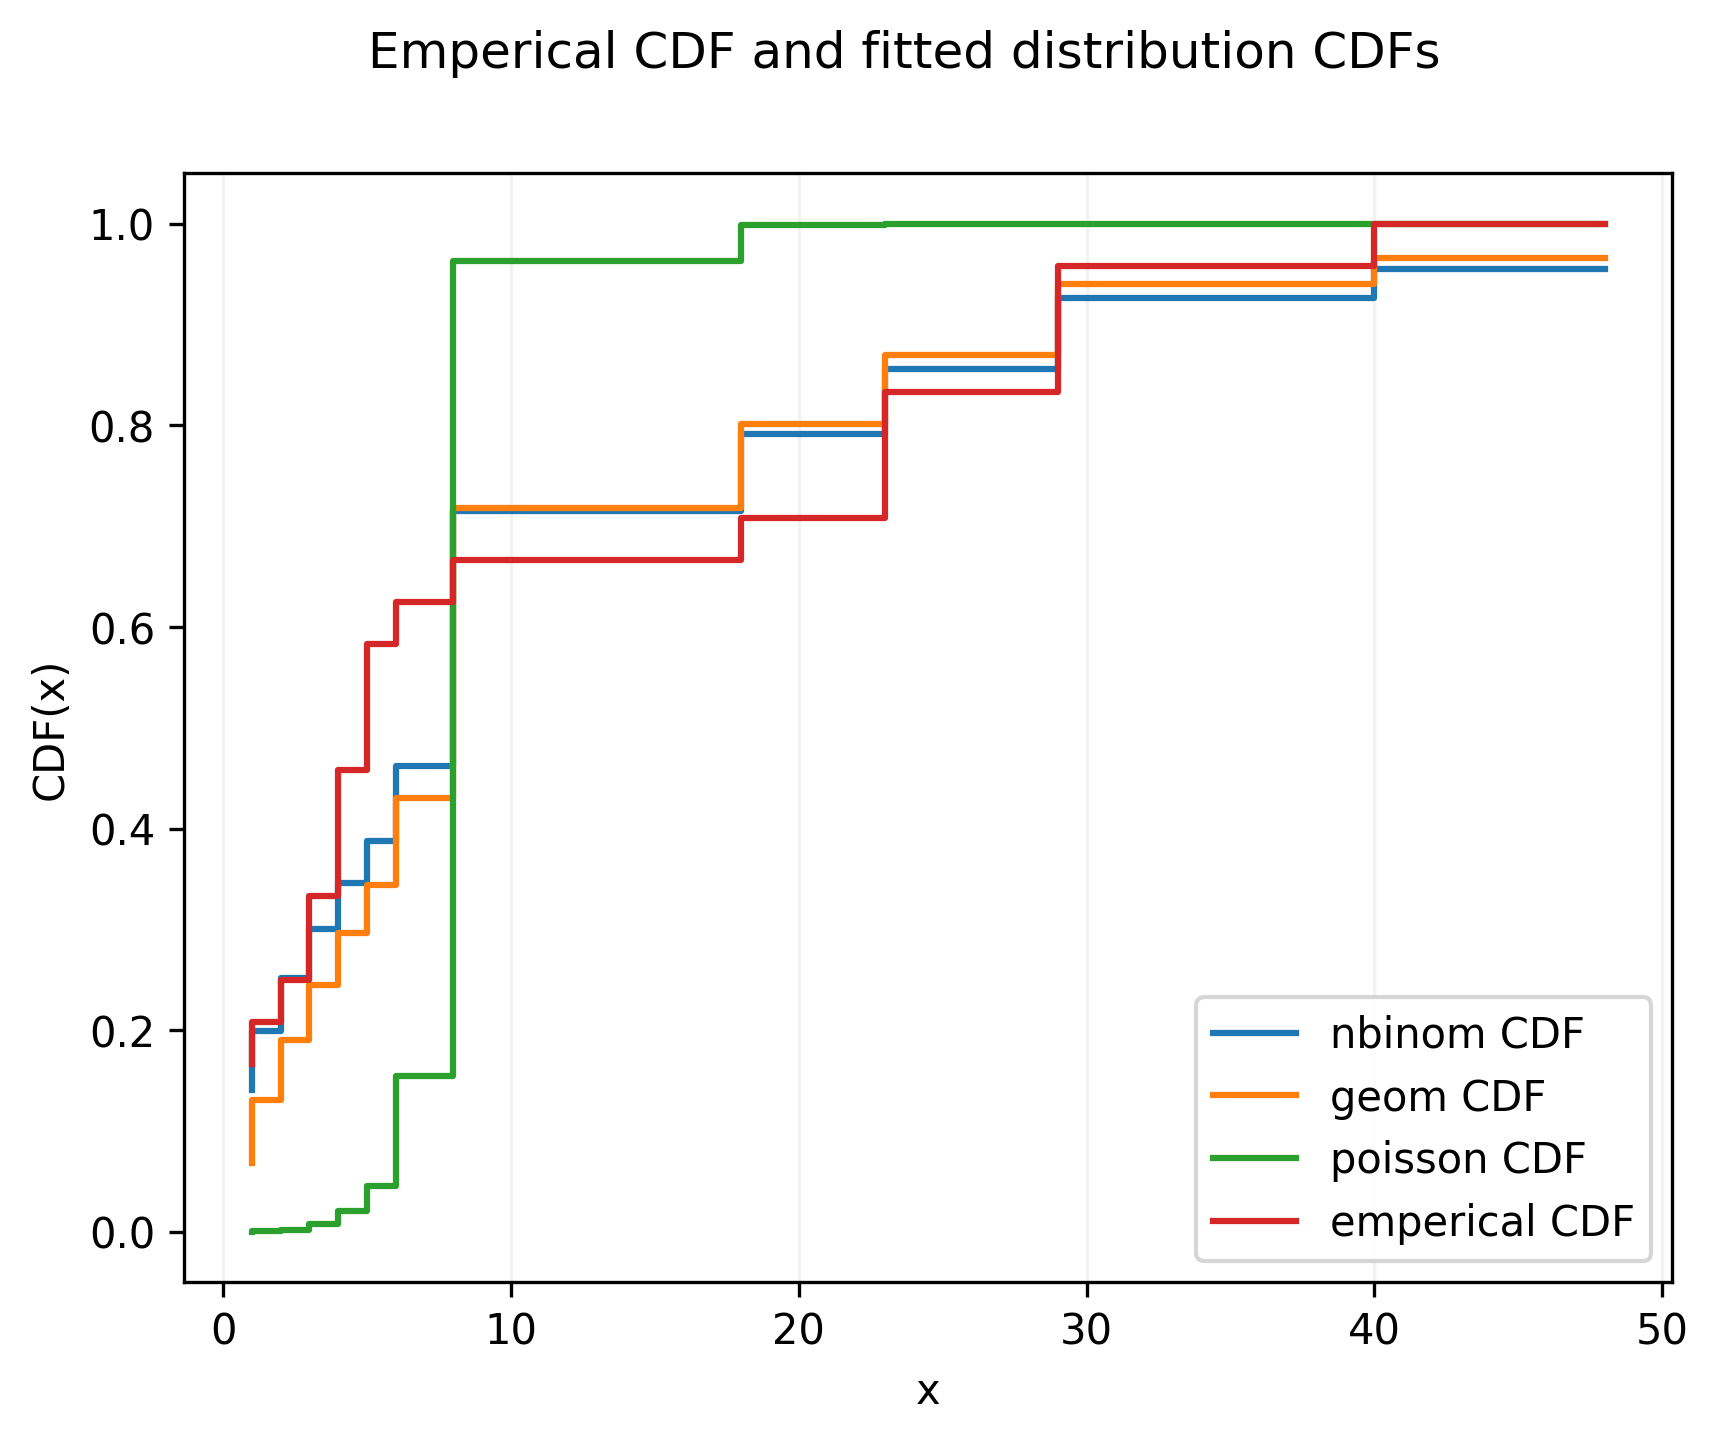
\includegraphics[width=.48\linewidth,valign=m]{CDF_compare_2005_I.ricinus_FV} & 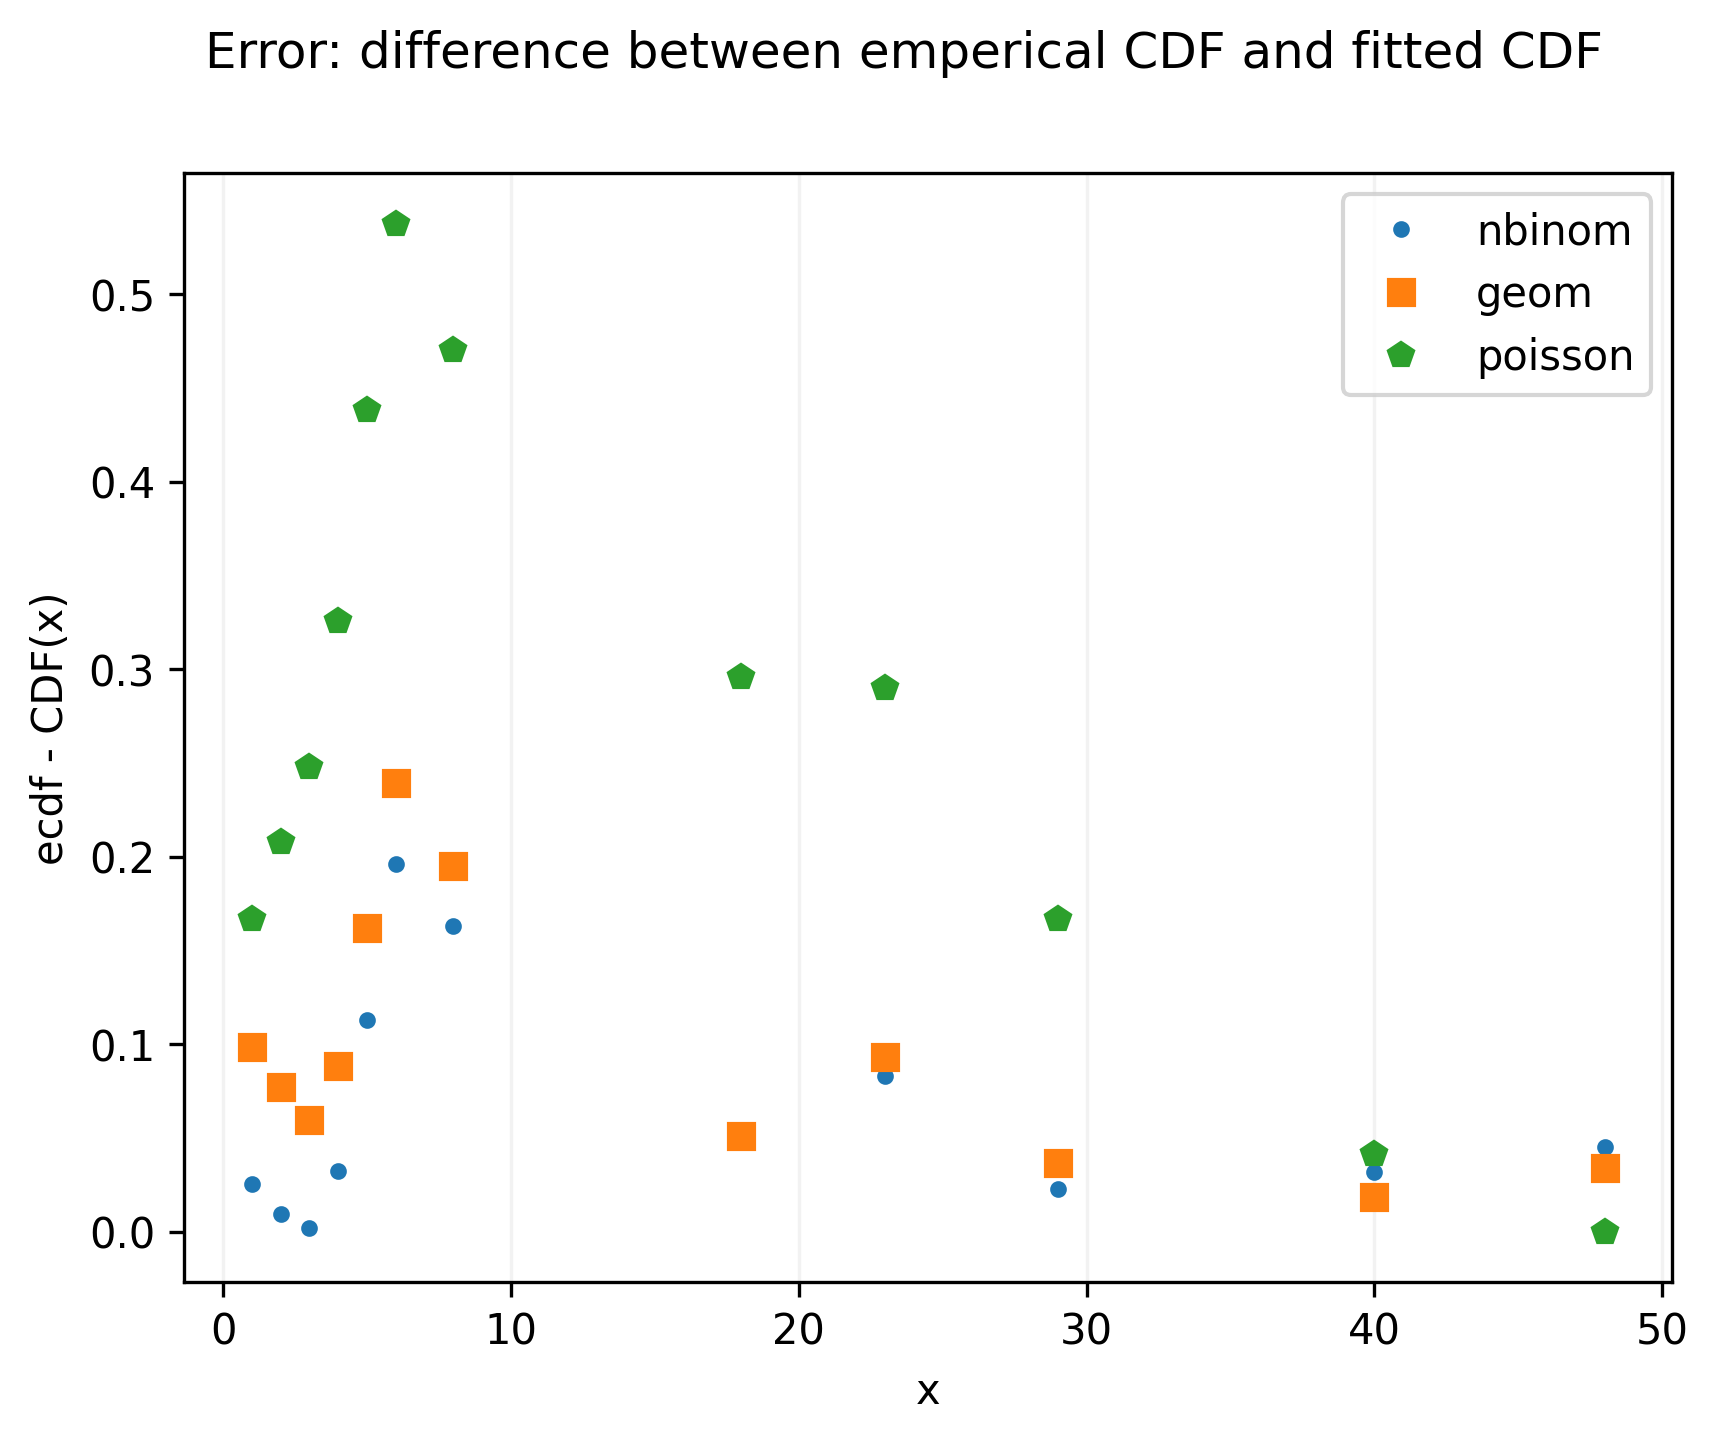
\includegraphics[width=.48\linewidth,valign=m]{CDF_errors_2005_I.ricinus_FV}
	\end{tabular}
	\caption{Discrete probability distributions fitted to the co-aggregation data $ X $ for \textit{I. ricinus} found on \textit{field voles} in \textit{2005}.}
	\label{fig:kielder_2005_iricnus_FV}
\end{figure}

\begin{figure}[h!]
	\centering
	\begin{tabular}{ll}
	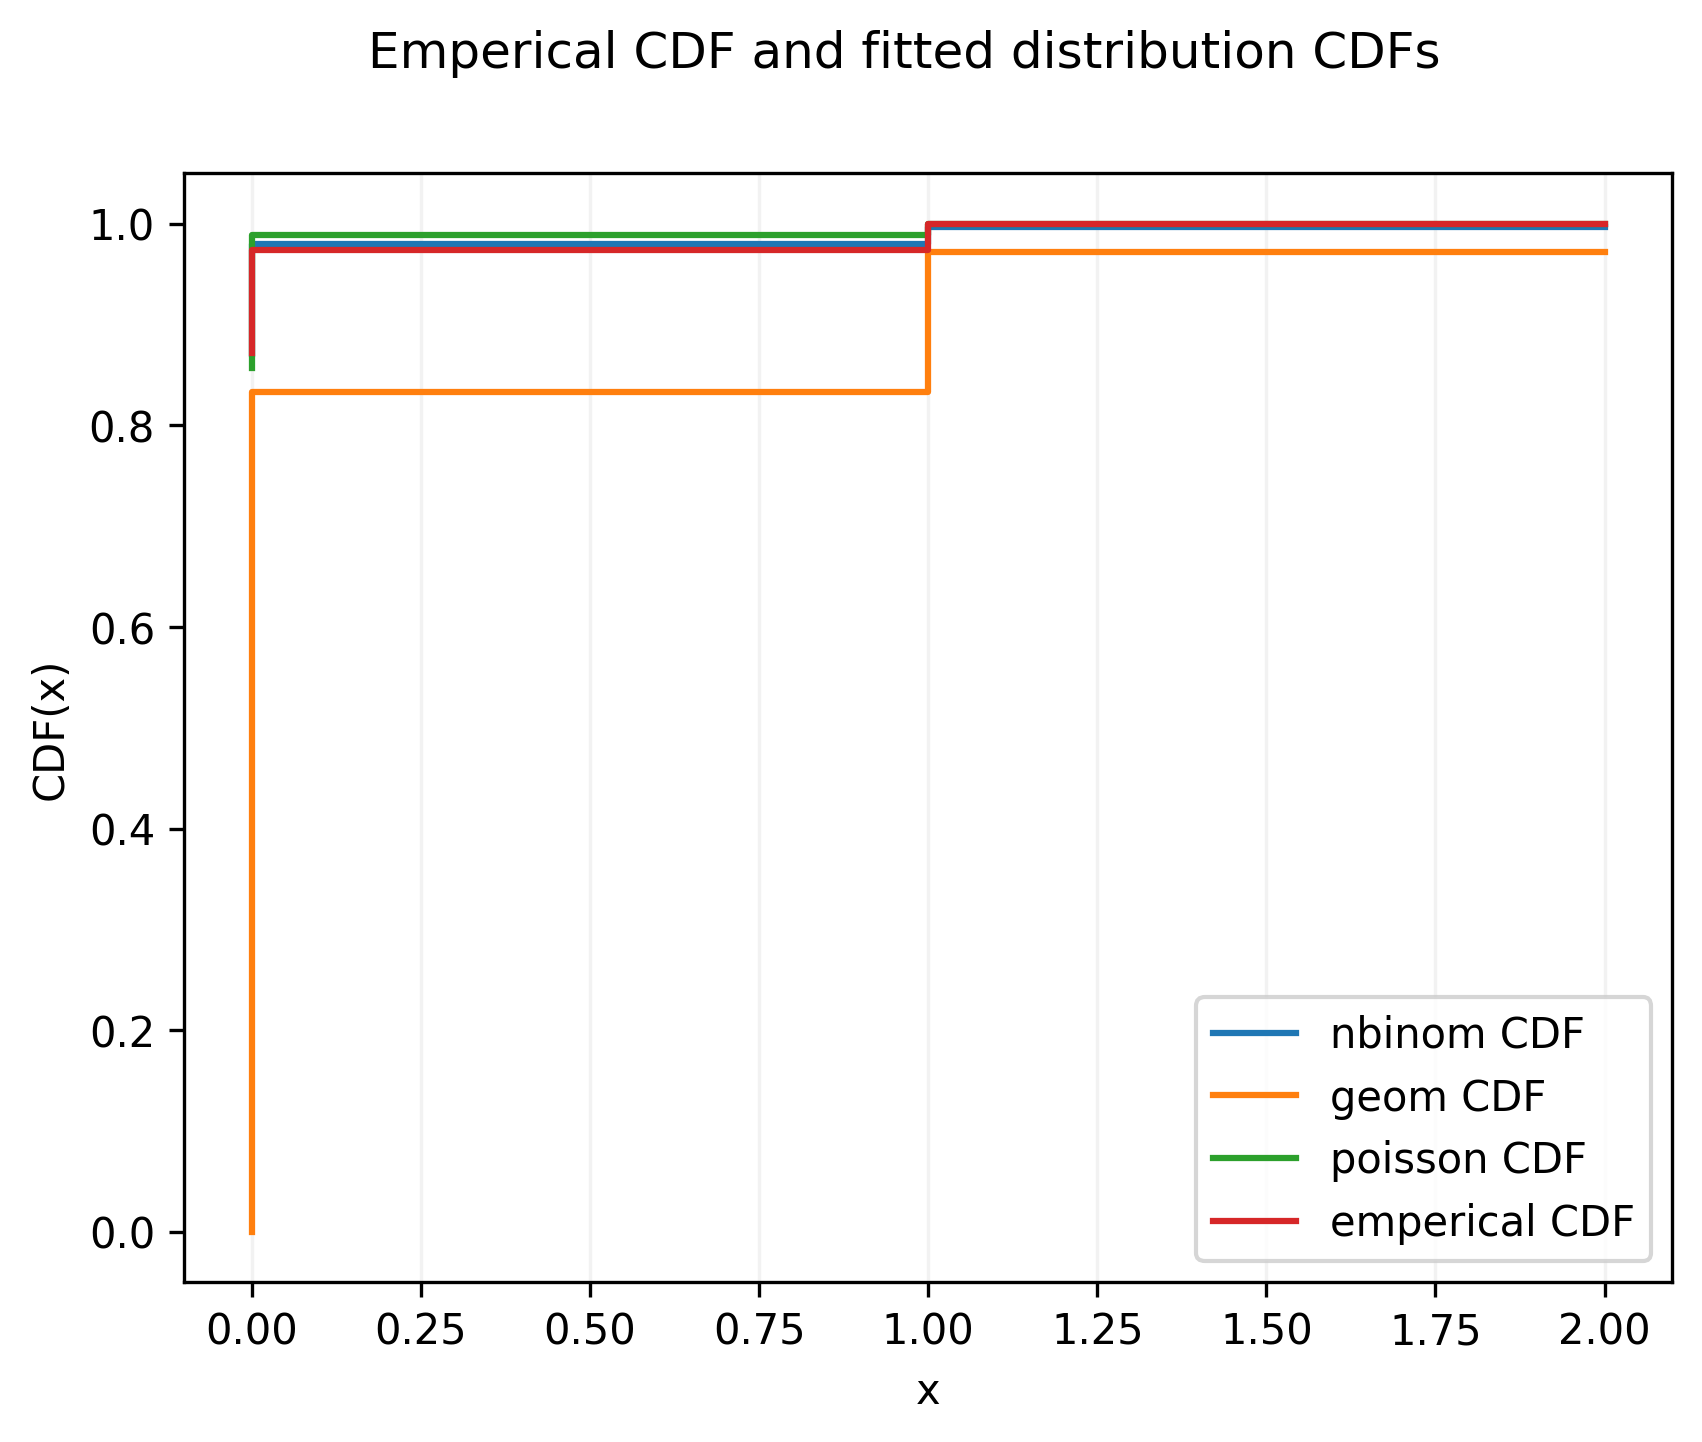
\includegraphics[width=.48\linewidth,valign=m]{CDF_compare_2005_I.trianguliceps_FV} & 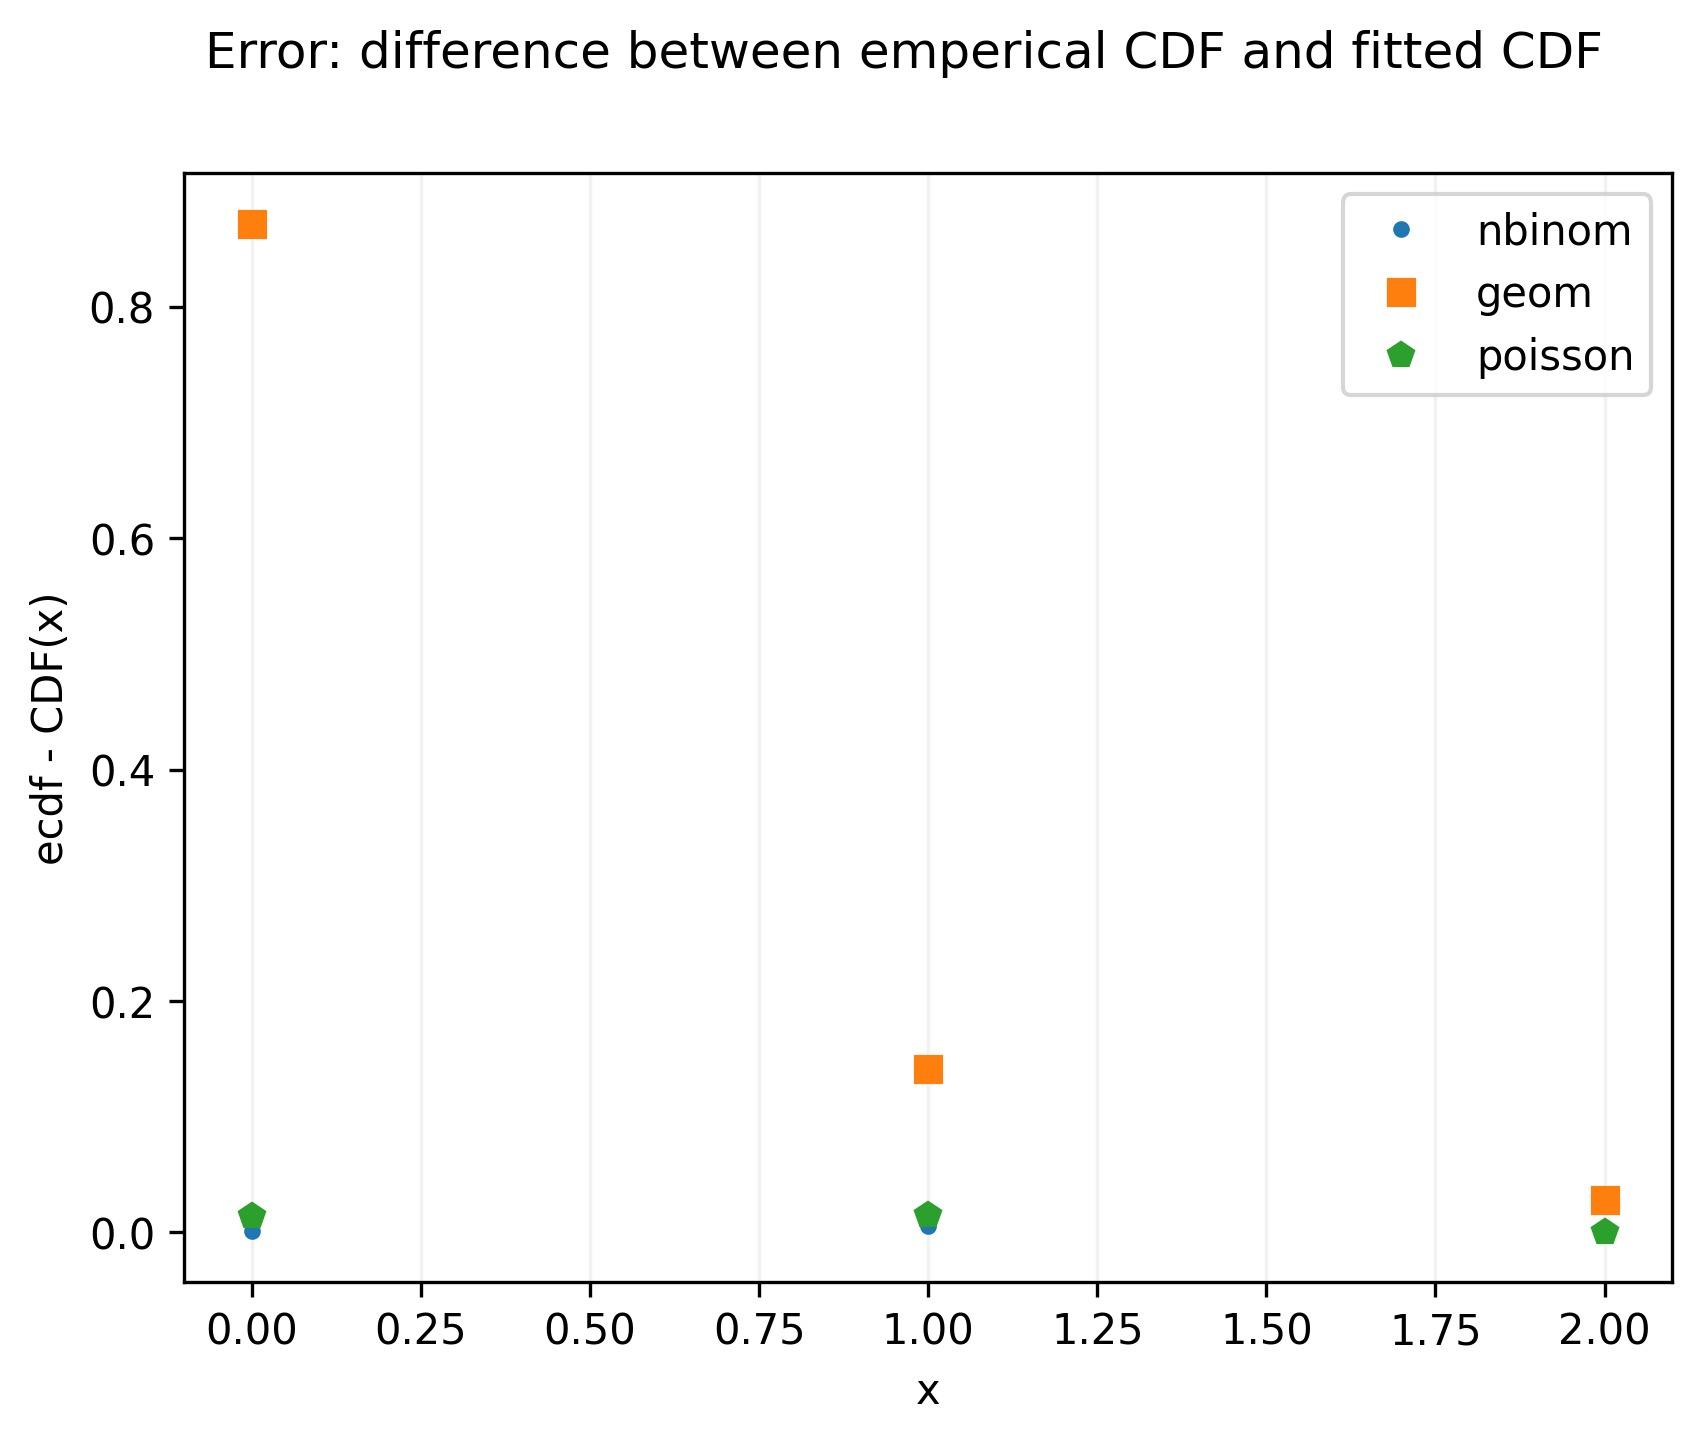
\includegraphics[width=.48\linewidth,valign=m]{CDF_errors_2005_I.trianguliceps_FV}
	\end{tabular}
		\caption{Discrete probability distributions fitted to the co-aggregation data $ X $ for \textit{I. trianguliceps} found on \textit{field voles} in \textit{2005}.}
	\label{fig:kielder_2005_itrianguliceps_FV}
\end{figure}

\begin{figure}[h!]
	\centering
	\begin{tabular}{ll}
	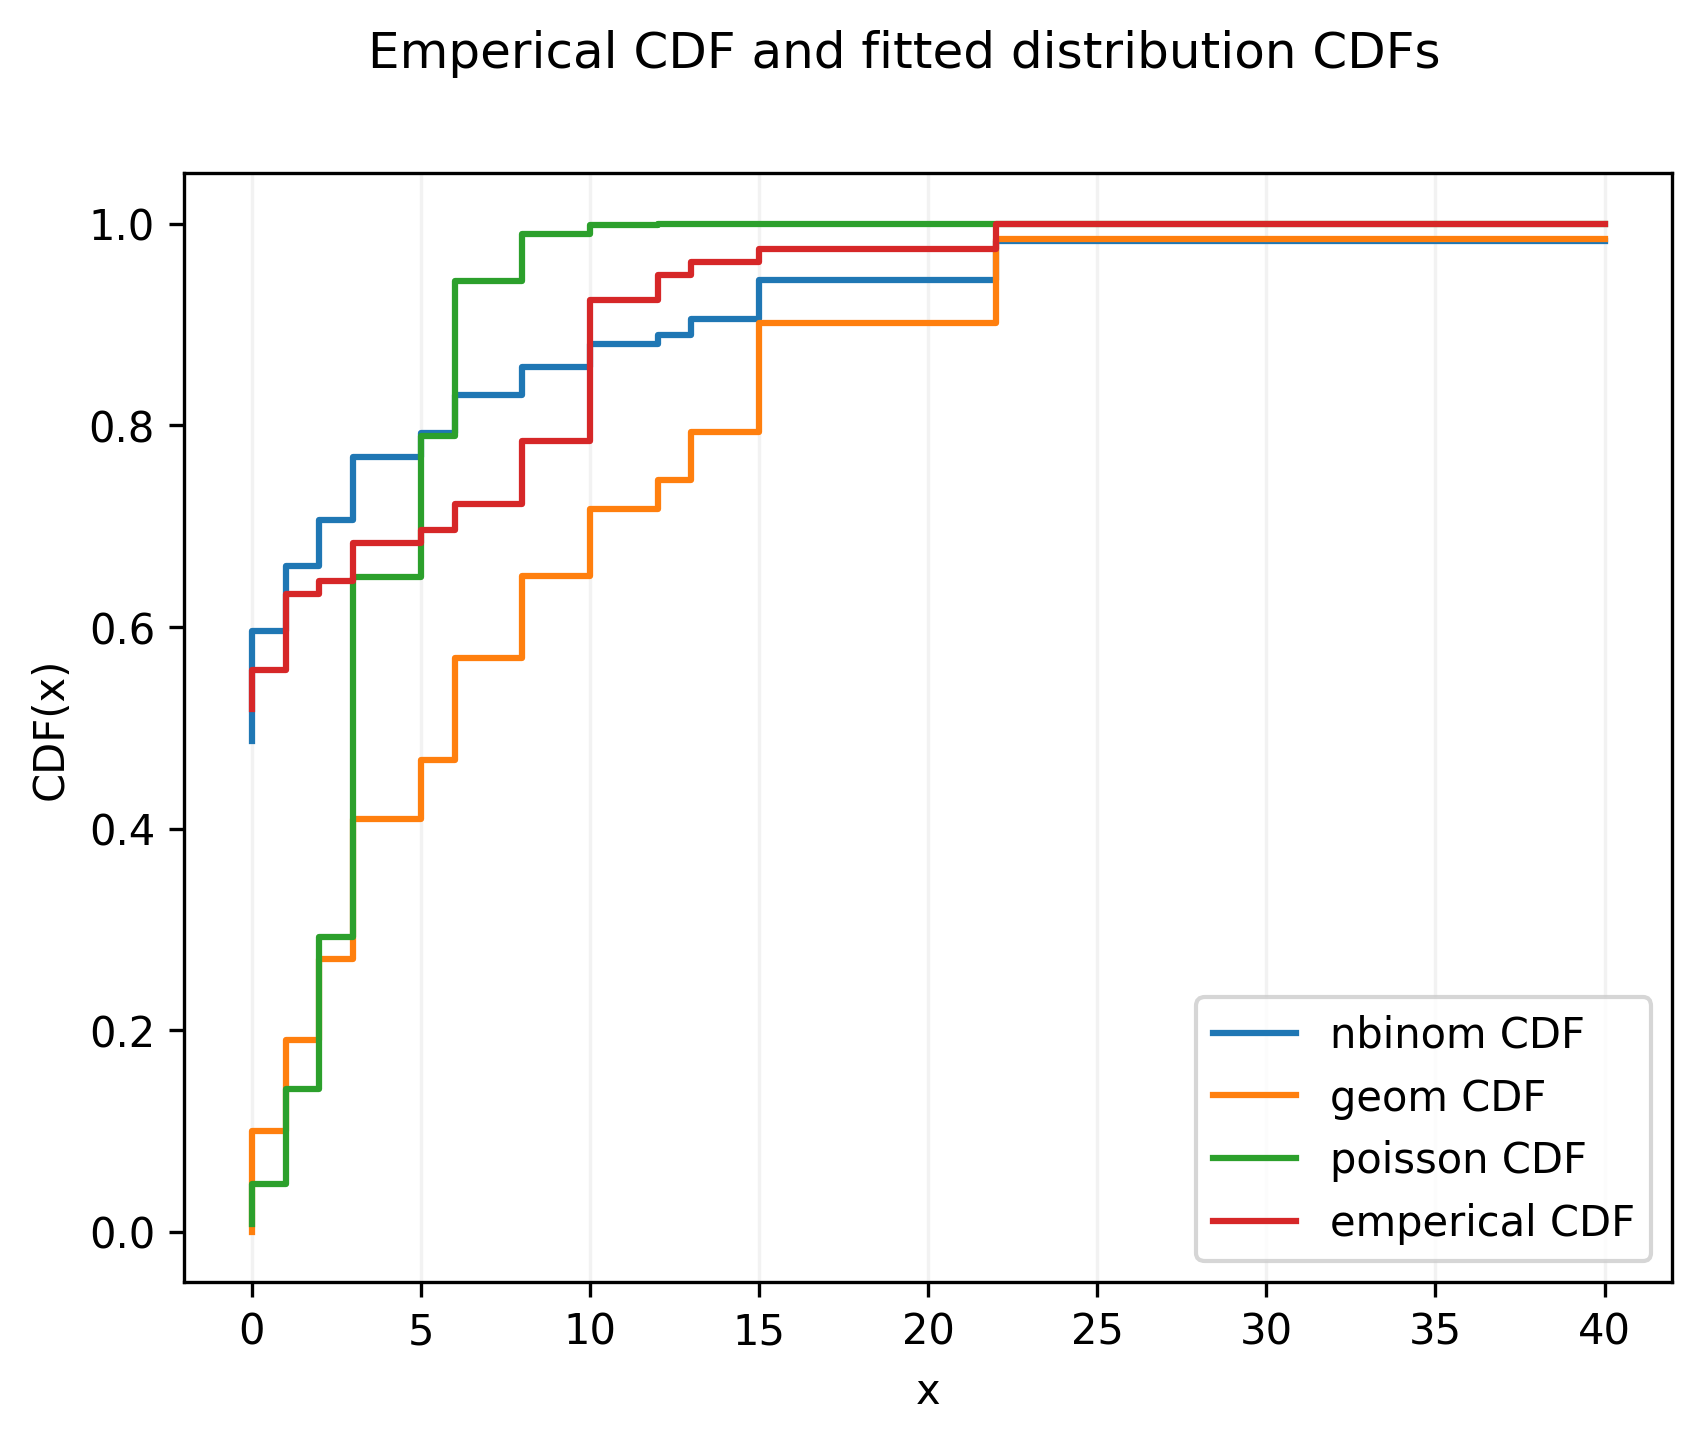
\includegraphics[width=.48\linewidth,valign=m]{CDF_compare_2005_I.trianguliceps_SA} & 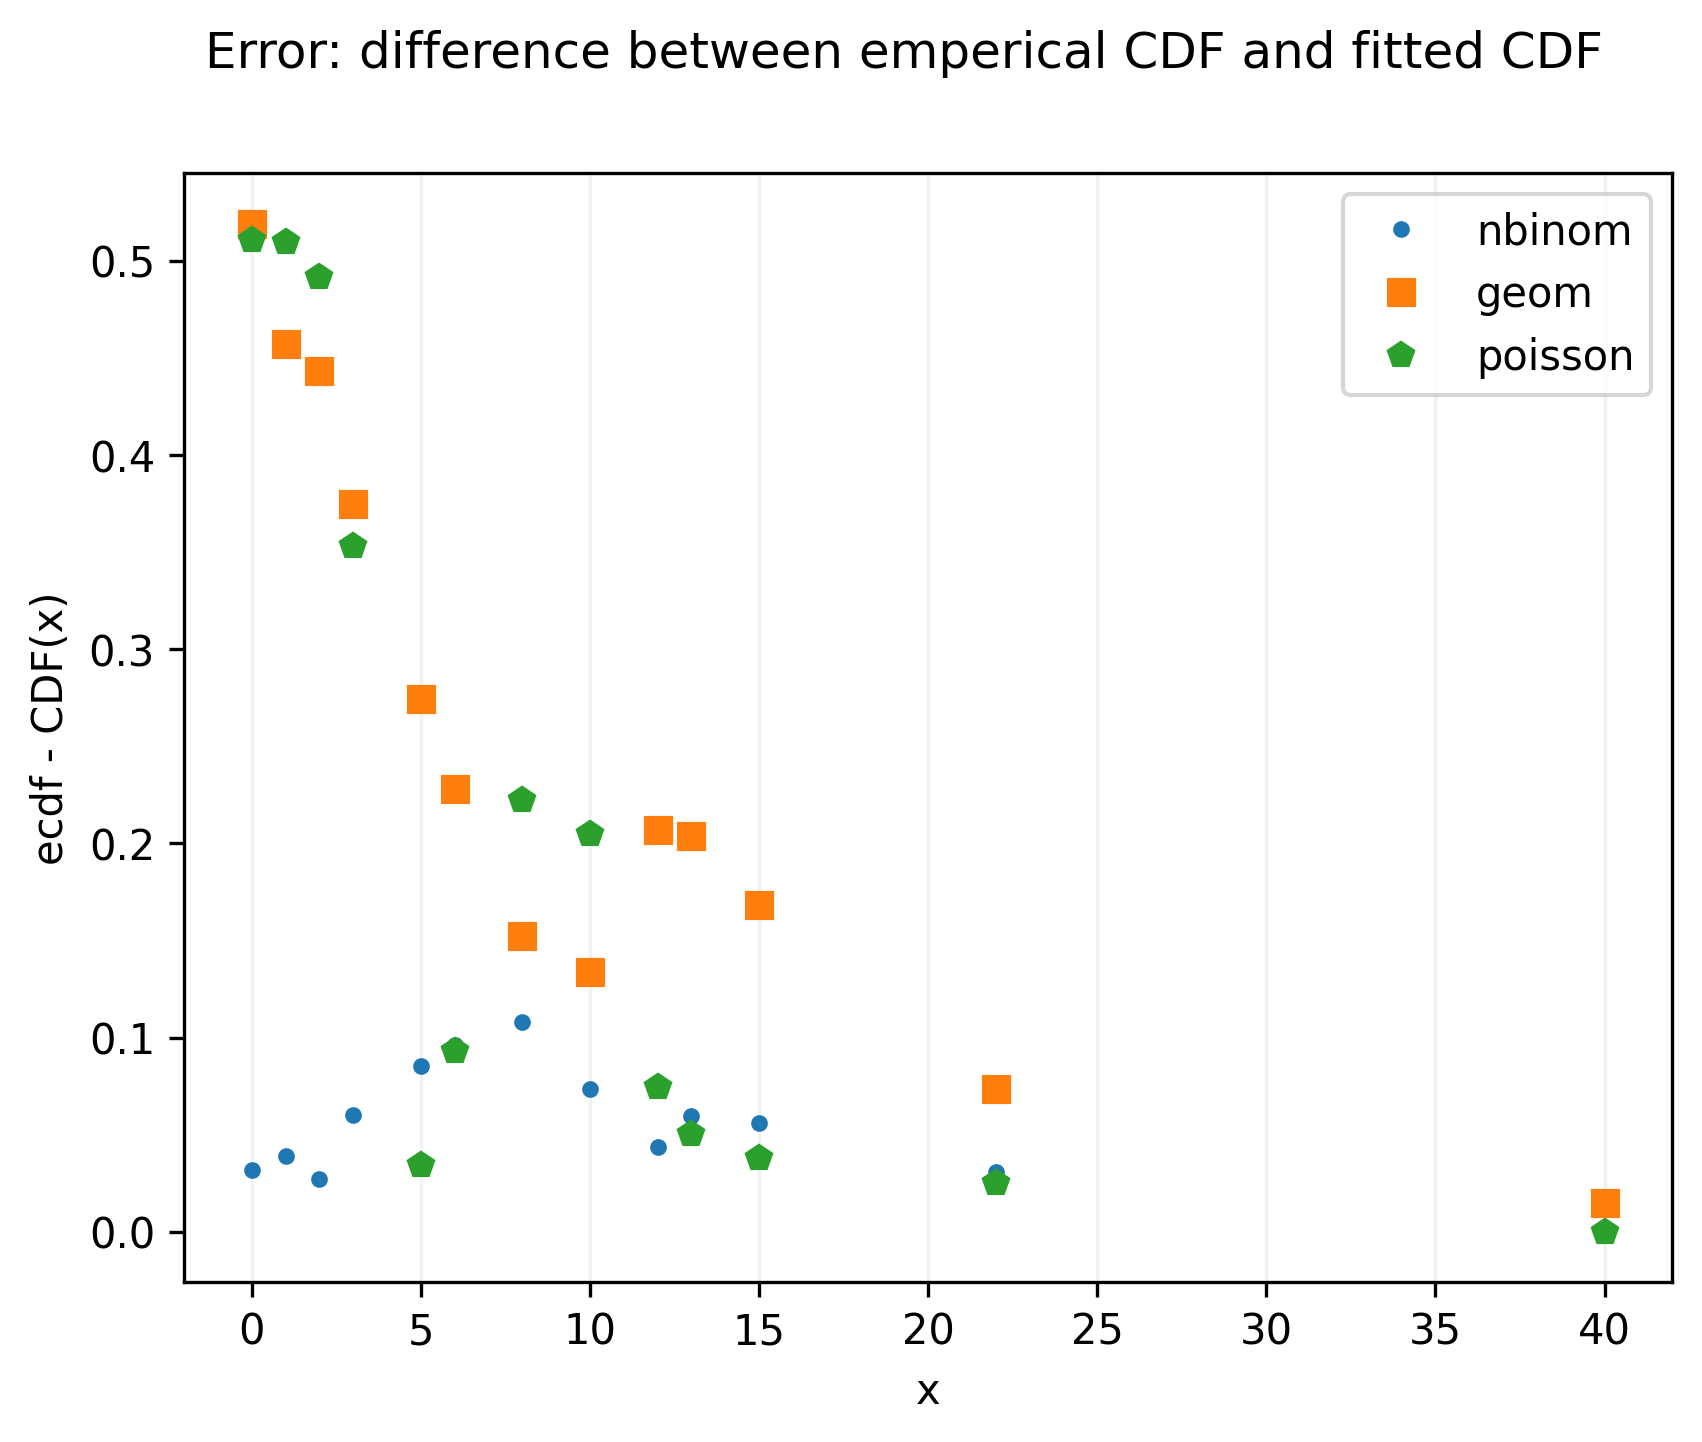
\includegraphics[width=.48\linewidth,valign=m]{CDF_errors_2005_I.trianguliceps_SA}
	\end{tabular}
		\caption{Discrete probability distributions fitted to the co-aggregation data $ X $ for \textit{I. trianguliceps} found on \textit{common shrews} in \textit{2005}.}
	\label{fig:kielder_2005_itrianguliceps_SA}
\end{figure}

To calculate goodness of fit, for each distribution and for each subset of data, we used AIC as did the Lloyd-Smith et al paper. The AIC method rewards the best-fitting models while penalising models by their number of parameters. In the sense that the negative binomial, Poisson and geometric distributions are models, the negative binomial's fit will be offset by its extra parameter, while the Poisson and geometric distributions each have just one parameter. REF DETAILS ABOUT PARAMS.

AIC for distributions' fit to co-aggregation data were calculated as:

\begin{align} \label{AIC}
    AIC &= 2K - 2\ln(L(\hat \theta | X)) \nonumber \\
    AIC_c &= AIC + \frac{2K(K+1)}{n-K-1}
\end{align}

For the Kielder Forest data, these $ AIC_c $ scores are presented in table \ref{tab:kielderAIC}. A point of difference is that Lloyd-Smith and others scaled their $AIC_c $ by subtracting the smallest value in each dataset, but the smallest value in all tick burden datasets used in this project is always $ 0 $.

\begin{table}[h!]
\centering
\begin{tabular}{|r|l|l|}
\hline
\multicolumn{1}{|l|}{Tick species}                                                              & Distribution      & $AIC_c $    \\ \hline
\multirow{3}{*}{\textit{\begin{tabular}[c]{@{}r@{}}I. ricinus\\ I. trianguliceps\end{tabular}}} & geometric         & $ \infty $ \\ \cline{2-3} 
                                                                                                & Poisson           & $ 4955 $   \\ \cline{2-3} 
                                                                                                & negative binomial & $ 2013 $   \\ \hline
\multirow{3}{*}{\textit{I. ricinus}}                                                            & geometric         & $ \infty $ \\ \cline{2-3} 
                                                                                                & Poisson           & $ 806 $    \\ \cline{2-3} 
                                                                                                & negative binomial & $ 332 $    \\ \hline
\multirow{3}{*}{\textit{I. trianguliceps}}                                                      & geometric         & $ \infty $ \\ \cline{2-3} 
                                                                                                & Poisson           & $ 3544 $   \\ \cline{2-3} 
                                                                                                & negative binomial & $ 1318 $   \\ \hline
\end{tabular}
\caption{Each subset of Kielder Forest data includes the common shrew and field vole species of vertebrates.}
\label{tab:kielderAIC}
\end{table}

\subsection{Fitted co-aggregation and offspring distributions}



\newpage

\section{Discussion}

\section{Conclusion}
 
\newpage

\nocite{*}

\section{References}
\printbibliography[heading=none]

\section{Appendix}
The code to generate all charts and figures used in this project is available in this Github repository: \url{https://github.com/JasonThomasData/maths_notes/tree/master/honoursProjectSrc}
TODO: create dedicated repo with README explaining how to run scripts.

\end{document}